\documentclass{article}
\usepackage{fullpage}
\usepackage{graphicx}
\usepackage[hidelinks]{hyperref}

\usepackage{color}
\usepackage{amsmath,amssymb,amsthm}
\usepackage{natbib}

\bibliographystyle{plainnat}


\newcommand{\R}{\mathbb{R}}
\newcommand{\Q}{\mathbb{Q}}
\newcommand{\Z}{\mathbb{Z}}
\newcommand{\N}{\mathbb{N}}

\renewcommand{\P}{\mathbb{P}}
\newcommand{\E}{\mathbb{E}}
\newcommand{\var}{\mathop{\mbox{Var}}}
\newcommand{\cov}{\mathop{\mbox{cov}}}
%\newcommand{\det}{\mathop{\mbox{det}}}
\newcommand{\deg}{\mathop{\mbox{deg}}}
\newcommand{\supp}{\mathop{\mbox{supp}}}
\newcommand{\sgn}{\mathop{\mbox{sgn}}}

\newcommand{\bone}{\mathbf{1}}
\newcommand{\st}{\,\colon\,}

% These macros are borrowed from TAOCPMAC.tex
\newcommand{\slug}{\hbox{\kern1.5pt\vrule width2.5pt height6pt depth1.5pt\kern1.5pt}}
\def\xskip{\hskip 7pt plus 3pt minus 4pt}
\newdimen\algindent
\newif\ifitempar \itempartrue % normally true unless briefly set false
\def\algindentset#1{\setbox0\hbox{{\bf #1.\kern.25em}}\algindent=\wd0\relax}
\def\algbegin #1 #2{\algindentset{#21}\alg #1 #2} % when steps all have 1 digit
\def\aalgbegin #1 #2{\algindentset{#211}\alg #1 #2} % when 10 or more steps
\def\alg#1(#2). {\medbreak % Usage: \algbegin Algorithm A (algname). This...
  \noindent{\bf#1}({\it#2\/}).\xskip\ignorespaces}
\def\kalgstep#1.{\ifitempar\smallskip\noindent\else\itempartrue
   \hskip-\parindent\fi
   \hbox to\algindent{\bf\hfil #1.\kern.25em}%
   \hangindent=\algindent\hangafter=1\ignorespaces}

\newcommand{\algstep}[3]{\kalgstep #1 [#2] #3 }
\newenvironment{taocpalg}[3]{%
\vspace{1em}%
\algbegin Algorithm #1. ({#2}). #3 }
{\vspace{1em}}

\newcommand{\randomuniform}[0]{\mathcal{R}_U}
\newcommand{\randomdiscrete}[0]{\mathcal{R}_D}
\newcommand{\algref}[1]{#1}


\newcommand{\tskit}{{\texttt{tskit}}}
\newcommand{\tsinfer}{{\texttt{tsinfer}}}
\newcommand{\branch}{\mbox{Branch}} % branch stat
\newcommand{\branchp}{\mbox{Branch}_+} % polarised
\newcommand{\site}{\mbox{Site}} % site stat
\newcommand{\sitep}{\mbox{Site}_+} % polarised
\newcommand{\node}{\mbox{Node}} % node stat
\newcommand{\nodep}{\mbox{Node}_+} % polarised
\newcommand{\given}{\;\vert\;}

\newcommand{\treeseq}{\mathbb{T}} % tree sequence
\newcommand{\iw}{w} % sample (initial) weights
\newcommand{\tiw}{w_\text{total}} % total sample (initial) weights
\newcommand{\nw}{x} % subtree (node) weights
\newcommand{\aw}{{\bar x}} % allele weights

\newcommand{\Nt}{\mathcal{N}}  % node table
\newcommand{\Et}{\mathcal{E}}  % edge table
\newcommand{\prop}[1]{.\mbox{\texttt{#1}}} % property of a thing
% Not sure about this notation. Want to use i and o, but using normal
% math fonts would make things less clear, I think.
\newcommand{\indexin}[0]{\ensuremath{\mathbf{i}}}
\newcommand{\indexout}[0]{\ensuremath{\mathbf{o}}}
\newcommand{\plr}[1]{{\color{blue}\textbf{plr:} \it #1}}
\newcommand{\jk}[1]{{\color{red}\textbf{jk:} \it #1}}
\newcommand{\krt}[1]{{\color{green}\textbf{krt:} \it #1}}


\begin{document}

\title{
    Efficiently summarising relationships in large samples:
    a general duality between statistics of genealogies and genomes}
\author{Peter Ralph, Kevin Thornton, and Jerome Kelleher}
\maketitle

% \emph{Running head:} Genealogies and genomes

\krt{several refs seem missing}


%%%%%%%%%%
\section*{Abstract}

As a genetic mutation is passed down across generations,
it distinguishes those genomes that have inherited it from those that have not,
providing a glimpse of the genealogical tree relating the genomes to each other at that site.
Summaries of genetic variation therefore also describe the underlying genealogies.
Here we exploit this duality to create a method that efficiently computes single-site statistics
from population genetic data using the succinct tree sequence encoding
of genealogies and genome sequence.
We use the framework to provide efficient implementations of
many currently-defined statistics, and to suggest several new statistics.
The general approach aggregates ``sample weights'' up each marginal tree,
which are then summarised using a ``summary function'';
different statistics result from different choices of weight or function.
The results can be summarised in three different ways:
by \emph{site}, which corresponds to statistics calculated from genome
sequence;
by \emph{branch}, which gives the expected value of the site statistic
with a large number of mutations under the infinite-sites model;
or by \emph{node}, which summarises the contribution of each node in the tree to the statistics.
This formulation also makes it apparent what statistic of the underlying genealogical trees
each sequence-based statistic is estimating.  By using simulations to evaluate performance, we
show that calculating statistics from tree sequences is several orders of magnitude more efficient than
methods traversing the entire data matrix in terms of both run time and memory requirements.
We also use tree sequences inferred from the 1000 Genomes Project dataset,
to evaluate how well this duality between site and branch statistics holds
and to describe the temporal origin of some admixture statistics.


%%% OUTLINE
% 1. Framework and algorithms for computing general stats
%
%     * Framework:
%
%         - single-site stats are functions of the genotype vector
%         - in infinite sites, the genotype vector of a mutation is determined by the nodes below it
%         - ex: divergence as a sum over trees and branches
%         - ex: ancestry proportions
%         - general definition, using summary function of weights propagated up the tree
%             * recursion relating weights on nodes of two forests that differ by a branch
%
%     * Review of tree sequences (quick)
%
%     * Algorithms:
%
%         - weight propagation across tree differences
%         - count by node length ("Node Statistics")
%         - count by branch area ("Branch Statistics")
%         - count by site ("Site Statistics")
%         - note on outputs (by node, by site, in windows)
%
% 2. Examples: in sections, one of each type of output
%
%     - ancestry proportions
%     - list of standard summary statistics: divergence, Fst, f4, covariance
%         * performance for one of these
%     - PCA: Krylov method
%         * performance
%
% 3. Correspondence to tree statistics
%
%     - math: in infinite sites, neutral model, E[site] = branch
%     - plot from simulation showing branch stats are less noisy versions of the site stats
%     - show time profile of PC1 as computed from rare variants and common variants



%%%%%%%%%%%%%%%%%%%%%%%
\section*{Introduction}

It was once a major undertaking to collect data sufficient to estimate a single summary
of the many genetic relationships between the individuals of a sample,
e.g., to estimate $F_{ST}$ between two populations using a dozen allozymes.
\jk{Citation?}
Today's vast quantity of whole-genome sequence
makes it possible to confidently estimate many more properties of genealogical relationships
in local regions of genomes \citep{stankowski2019widespread,fst_landscapes},
or between individuals rather than populations \citep{individual_stats}.
Computation is beginning to be a major problem:
genetic data on the scale of the UK Biobank~\citep{bycroft2018genome},
for instance, might have 500K individuals genotyped at 10M loci,
resulting in a genotype matrix of $5 \times 10^{12}$ entries.
Computing a single summary from this matrix is still relatively quick,
once loaded into memory,
but for many applications we are now interested in computing a large number of statistics,
or iteratively refining a single computation.
Furthermore, even larger datasets are being collected,
and millions of whole genomes will soon be available. In this case the
genotype matrix simply cannot fit into memory, and complex distributed
computations are required to calculate population genetic statistics.

Fortunately, the genotype matrix is not the only way to encode genetic data.
The \emph{succinct tree sequence} (or \emph{tree sequence}, for brevity) is a data
structure that efficiently encodes the genealogical trees describing how a set of
individuals are related to each other at each point along their genome.
It was introduced in the context of coalescent
simulation~\citep{kelleher2016efficient}, and led to scalability increases of
several orders of magnitude over existing methods. The methods were subsequently extended
and refined for forwards-time
simulations~\citep{kelleher2018efficient,haller2018tree}, with similar efficiency gains.
Recent work~\citep{kelleher2019inferring} has shown that tree sequence algorithms can
also be used to massively increase the scalability of methods for inferring
genome-wide genealogies, and making it possible to infer trees for millions of
samples.
The key to the remarkable scalability and efficiency of tree sequence
algorithms is the way that shared structure in adjacent trees along the genome is encoded.
As one looks across the genome, genealogies change at recombination breakpoints in ancestors.
However, nearby trees tend to share a lot of common structure,
and single genealogical relationships (e.g., individual $x$ inherits from individual $y$)
are often shared across relatively long distances,
which manifest as shared \emph{edges} across many adjacent trees in the tree sequence.
This redundancy can be exploited to store genome sequence and the
associated genealogical relationships very compactly, while also
allowing us to to compute several population genetics statistics
efficiently~\citep{kelleher2016efficient}.
This paper generalizes the approach to a much broader class of statistics.

Naturally, the genealogical perspective on population genetics statistics has a long history.
The sequence of trees describing genealogical relationships as one moves along the genome
are also described by the Ancestral Recombination
Graph~\citep{griffiths1991two,griffiths1996ancestral,rasmussen2014genome}.
These genealogical trees can be fairly precisely inferred in nonrecombining regions
\citep{felsenstein2004inferring},
as for instance the mitochondria,
and substantial theoretical work has been done in the context of phylogenetics \citep{semple2003phylogenetics}.
% describing how each mutation gives a small piece of information about the tree at that site
% However, population genetics has the task of summarizing relationships across \emph{many} trees,
% each only partially known because mutations are sparse in the data.
The basic relationship between tree shape and summaries of genetic variation
is that if mutations are neutral then the expected number that occur on a given branch
is proportional to the length of that branch,
thus establishing a duality between genealogical and genetic summaries,
a fact used extensively in deriving properties of statistics in models of random mating
\citep[e.g.][]{tajima1983evolutionary,tavare1984lineofdescent,fu1995statistical}.
The fact that the duality applies regardless of the underlying demographic model was also used
\citep[e.g.][]{gillespie1979evolutionary,hudson1983properties,slatkin1991inbreeding,mcvean2002genealogical,ralph2019empirical},
but only recently have datasets made it possible to move beyond a few numerical summaries.

% summary
In this paper, we study only ``single-site'' genetic statistics,
i.e., statistics of aligned genome sequence that can be expressed as averages over values computed
separately for each site,
leaving other statistics (e.g., pairwise statistics such as linkage disequilibrium
or haplotype statistics) for later work.
The methods we describe are implemented, tested, and validated in the \tskit{} library,
which is available as an open-source Python package at \url{https://github.com/tskit-dev/tskit}.


%%%%%%%%%%%%%%%%%%%%%%%
\section*{Framework and statistics}

\jk{These two intro paragraphs aren't working for me. There's too many
parenthetical comments, mixing high-level overview with getting into
the weeds. Does the first para actually help? Perhaps we're just confusing
people by talking about the AFS here?}
Many population genetic summary statistics can be defined using the allele frequency spectrum
of a collection of homologous sequences.
Concretely, write $p_i(a)$ for the frequency of allele $a$ at a site $i$,
and $h(p)$ for the allele frequency spectrum
--- i.e., the number of alleles whose frequency is $p$ in our sample ---
and suppose that for some function $f()$, we want to compute $\sum_p h(p) f(p)$.
(For instance, mean genetic diversity is computed with $f(p) = p (1-p)$.)
Since this is a simple sum over sites,
we can compute this by summing over the $L$ loci, as
\begin{align*}
    \sum_p h(p) f(p) = \sum_{i=1}^L \sum_a f(p_i(a)).
\end{align*}
(Note that since the ancestral allele is included, this function is invariant to relabeling of alleles.)
If we know where each mutation has occurred on the genealogy,
we can easily find the frequency of the corresponding allele by counting how many samples
inherit from that mutation in the tree (and accounting for those that subsequently mutate).

% 2-3 sentances of intro before this?
Roughly speaking, to compute a statistic we will
propagate ``weights'' additively up each tree,
summarize these weights on each branch with a ``summary function'',
and aggregate these summaries to produce statistics.
For instance, we could calculate how many of a certain set $A$ of samples
inherit from a particular edge in a tree
by (a) assigning each of these samples weight 1 (and other nodes weight zero), then
(b) finding the total weight of all nodes in the subtree inheriting from that edge.
Figure~\ref{fig:divergence_diagram} shows a simple example of these procedures
of propagating weights up a tree and summarising them,
used to calculate mean sequence divergence over a short sequence spanned by a single tree.

We now begin to formalize these notions with definitions.
In a tree sequence, each haplotype, modern or ancestral, is associated with a \emph{node},
and the trees at each position along the genome have vertexes labeled by these nodes.
A tree sequence describes the relationships between a special set of nodes, the \emph{samples},
that appear in the trees at every point along the genome.
The other (non-sample) nodes may not appear in every tree,
as for instance if a portion of an ancestor's genome was not inherited by any of the samples.

\begin{definition}[Sample and subtree weights] \label{defn:weights}
    A list of \emph{sample weights} $\iw$ assigns a numeric value $\iw(v)$
    to every sample node.
    Given these and a tree $T$,
    the \emph{subtree weight} $\nw_T(u)$ for a node $u$ is the sum of all sample weights
    of every sample node that is descended from $u$ in the tree (including $u$, if it is a sample):
    \begin{align*}
        \nw_T(u) = \sum_{v \,:\, v \le_T u} \iw(v) ,
    \end{align*}
    where $v \le_T u$ if $u$ is on the path from $v$ to root in the tree $T$.
    The \emph{total weight} is the sum of the weights over all samples:
    $\tiw = \sum_v \iw(v)$, which is the subtree weight of the root of any tree
    that contains all samples.
\end{definition}

We allow vector-valued weights,
i.e., $\iw(v)$ may be a vector $(\iw_1(v), \ldots, \iw_m(v))$,
so that when summarising we have access to more than one aspect of each subtree.

\begin{definition}[Summary function]
    For a set of $k$-dimensional weights with total weight $\tiw$,
    a summary function is a real-valued function $f(w_1, \ldots, w_k)$
    with the property that $f(0) = f(\tiw) = 0$.
\end{definition}

The requirement that $f(0) = f(\tiw) = 0$ is for consistency,
so that statistics do not depend on portions of the tree either not ancestral to any of the samples or ancestral to all
of them.
% Below, in section XXX, we describe how to efficiently
% maintain a list of the weights of the subtrees inherit from each node
% as we iterate through the tree sequence.

\begin{figure}
    \centering
    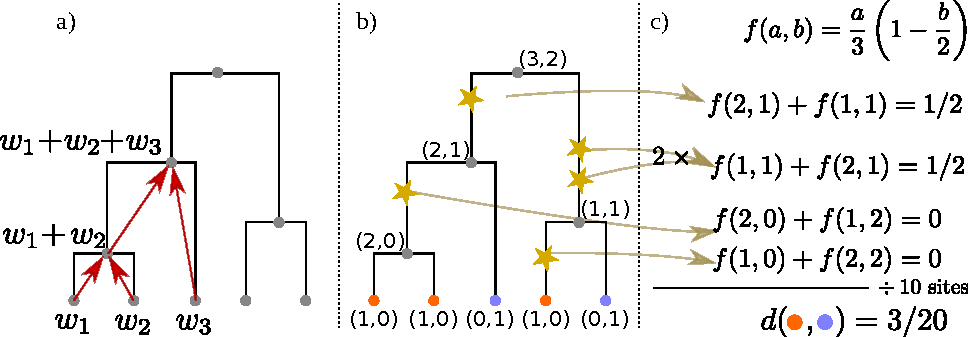
\includegraphics{figures/divergence_diagram}
    \caption{
        An example of computing sequence divergence between red nodes and blue nodes
        from seven mutations at distinct sites in a sequence of length 10 using the tree.
        The summary function, $f(a,b) = (a/3)(1-b/2)$ gives the probability that
        an allele found in $a$ of the red nodes and $b$ of the blue nodes is present in
        a randomly chosen red node but not in a randomly chosen blue node.
        \textbf{(a)} Weights are assigned to each subtree by adding together the weights of any children,
        plus the weight of the node itself, if it is a sample.
        \textbf{(b)} In this example, subtree weights $(a,b)$ record how many red nodes ($a$)
        and how many blue nodes ($b$) lie in that subtree.
        \textbf{(c)} The summary function shown is applied to both the weight of the subtree
        and the remaining weight of each mutation,
        so for instance the mutation above the node with weights $(2,1)$
        contributes $f(2,1) + f(1,1) = 1/3 + 1/6 = 1/2$.
        The final value for divergence is the sum of these values divided by 10,
        the total number of sites.
        \label{fig:divergence_diagram}
    }
\end{figure}


%%%%%%%%%%%%%%%%%%
\subsection*{Tree sequences}

Before defining the different classes of statistic,
it will help to establish a little more notation.
A tree sequence efficiently describes how a set of $n$ sampled chromosomes
are related to each other along a (linear) genome of length $L$ \citep{kelleher2016efficient,kelleher2018efficient}.
% These trees are highly correlated,
% a fact which allows them to be stored and processed very efficiently,
% as described in \citet{kelleher2018efficient}.
From the tree sequence can be extracted a sequence of trees,
$\treeseq = (T_1, T_2, \ldots, T_{n(\treeseq)})$
and a sequence of breakpoints $0 = a_0 < a_1 < \cdots < a_{n(T)} = L$,
where $T_k$ describes the genealogical relationships of the samples
over the segment of genome between $a_{k-1}$ (inclusive) and $a_k$ (exclusive).
We say that tree $T_k$ \emph{covers} the (half-open) segment $[a_{k-1}, a_k)$,
and call the length of this segment its \emph{span}, denoted $L_k = a_k - a_{k-1}$.
We refer to the branches in each tree using the most recent node,
so for instance a branch between an ancestor $v$ and descendant $u$
is associated with the node $u$.
The \emph{length} of this branch is the difference in birth times of $v$ and $u$,
and is denoted $\beta_T(u)$.
Note that although the same parent-child relationship may exist across many adjacent trees
(this is called an ``edge''),
rearrangements of genealogical relationships due to recombination
can cause the precise set of samples that inherit from that edge to differ across trees.


%%%%%%%%%%%%%%%%%%
\subsection*{Node statistics}

Perhaps the most natural way to summarise weights on the tree
is simply to examine the values at each node.
This would allow us, for instance, to
count the number of samples that inherit from each node in the tree.
Averaged across trees,
this tells us, for each node, what proportion of the sample's genomes were inherited from that node.
Motivated by this, we define the
\textbf{node statistic} for node $u$
associated with summary function $f()$ and sample weights $\iw$
to be the sum of $f()$ applied to the weight of the subtree inheriting from node $u$
and to the remaining weight,
averaged across the genome:
\begin{align}
    \node(f, \iw)_u
    =
    \frac{1}{L} \sum_{k=1}^{n(\treeseq)} L_k \left( f(\nw_{T_k}(u)) + f(\tiw - \nw_{T_k}(u)) \right).
\end{align}
The weight $\nw_{T_k}(u)$ is the subtree weight of node $u$ in the tree $T_k$,
and $\tiw - \nw_{T_k}(u)$ is the sum of all weights \emph{not} in the subtree of $u$ in $T_k$.
% i.e., the length of the segment of genome that the tree extends for.
% If this is computed over only a ``window'' of the genome
% then $L_k$ is replaced by the length of the portion of that window
% that $T$ extends for.

\paragraph{Polarisation}
The node statistic defined above is appropriate for statistics such as nucleotide diversity, which is a function
of all alleles at given variable site.  For other statistics, one is only concerned with the derived state(s)
at a site, and we may define a \emph{polarised} node statistic without the second term from our previous definition:

\begin{align}
    \text{(polarised)} \qquad
    \nodep(f, \iw)_u
    =
    \frac{1}{L} \sum_{k=1}^{n(\treeseq)} L_k f(\nw_{T_k}(u)) .
\end{align}

We will use weights that count number of samples inheriting from each node
sufficiently often that we give them a special name --
for a subset set $S$ of samples,
the \emph{indicator weights of $S$} are the sample weights $\bone_S$ with
$\bone_S(u) = 1$ if $u \in S$ and $\bone_S(u) = 0$ otherwise.

\begin{example}[Ancestry proportions] \label{ex:ancestry_props}
    If $\iw$ are the indicator weights of the set $S$ of $n$ samples,
    then $\nw(u) / n$ is the proportion of the samples in $S$ that inherit from $u$.
    Therefore, if $f(x) = x / n$,
    then $\nodep(f, \iw)_u$ is the proportion of the genomes of $S$
    that are inherited from (ancestor) $u$.
\end{example}

Node statistics only make sense in the context of the tree sequence,
but provide a useful bridge to the next type of statistic,
which are defined directly in terms of the genotypes.


%%%%%%%%%%%%%%%%%%
\subsection*{Site statistics}

Now we describe how to compute statistics from \emph{genomes} using this framework.
To do this, we assume that the genetic variation data is embedded in a tree sequence,
but the trees are used only for efficiency --
the results will not depend on the trees in any way
(with the only exception being if the ancestral allele is assumed to be known, as discussed below).

The summaries we defined above for each node in each tree
extend nicely to genetic variants
-- just as a node weight contains information about which samples inherit from the node and which are not,
so we can summarise patterns of genetic variation by summing up weights of all samples
that carry a given allele.
So, we define \emph{allele weights} to be
the total weight of all sample nodes who have inherited that allele.

\begin{definition}[Allele weights]
    The \emph{allele weight} for allele $a$ at site $j$ is the sum of the weights
    of all sample nodes inheriting this allele:
    \begin{align*}
        \aw_j(a) = \sum_{v \st g_j(v) = a} \iw(v) ,
    \end{align*}
    where the sum is over all sample nodes $v$ for which
    $g_j(v)$, the allele carried by node $v$ at site $j$, is equal to $a$.
\end{definition}

If there has been only one mutation at the site,
then $\aw_j(a)$ is equal to the weight of the subtree inheriting from the mutation that produced $a$.
More generally, $\aw$ is not necessarily equal to a subtree weight
but is easily computable from them.

Using allele weights,
we define the \textbf{site statistic} of site $j$ computed using a summary function $f()$
and a set of sample weights $\iw$
to be the sum of $f()$ applied to each of the allele weights:
\begin{align}
    \site(f, \iw)_j
    &=
    \sum_{a} f(\aw_j(a)) ,
\end{align}
where the sum is over all unique alleles at site $j$.

Of course, we often want to summarize statistics across regions of the genome (``windows'').
To do this, we overload notation somewhat and use a subscript $[i,j)$ to denote an average
over the corresponding portion of the genome:
\begin{align}
    \site(f, \iw)_{[i,j)}
    &=
    \frac{1}{j-i} \sum_{k=i}^{j-1} \site(f, \iw)_k
\end{align}
Since we have required $f(0) = f(\tiw) = 0$,
the sum will only be affected by polymorphic sites,
although the normalization is always by total number of sites, to allow comparison between regions.


In the definition above we simply sum over all alleles at each site.
However, sometimes it is useful to distinguish the \emph{ancestral} allele
(i.e., the allele at the root of the tree) from the remaining derived alleles.
This allows statistics in principle to differentiate ancestral from derived alleles,
information which is available in practice (albeit noisily),
and one way to make use of this information is to sum over only derived alleles.
Analogously to the above,
we say a site statistic is \textbf{polarised} if we do this,
defining
\begin{align} \label{eqn:site_polarised}
    \text{(polarised)} \qquad
    \sitep(f, \iw)_j
    &=
    \sum_{a \in D_j} f(\aw_j(a)) ,
\end{align}
where $D_j$ denotes the set of all alleles at site $j$ except the allele at the root of the tree.
Note that this may not be quite what is expected,
for instance, if there has been a back mutation to the ancestral allele at some point in the tree,
or if there have been mutations to distinct alleles on different parts of the tree
such that the ancestral allele is no longer present.
However, since these situations depend on multiple mutations occurring at a single site,
they are relatively rare in practice.

Having defined a general framework, we may now give concrete examples
of how to compute common summary statistics

\begin{example}[Nucleotide diversity] \label{ex:site_diversity}
    The nucleotide diversity of a group $S$ of $n$ samples
    is the average density of differences between pairs of samples,
    or equivalently, the average heterozygosity across positions.
    To calculate this statistic,
    % let $\iw_u = 1$ for $u \in S$ and $\iw_v = 0$ otherwise,
    let $\iw = \bone_S$,
    so that $\nw(u)$ gives the number of nodes in $S$ inheriting from $u$,
    and define
    \begin{align*}
        f(x) = \frac{x (n - x)}{n (n-1)} .
    \end{align*}
    Then $\site(f, \iw)_{[a,b)}$ is mean nucleotide diversity of $S$ in the region between $a$ and $b$.
\end{example}

\begin{example}[Nucleotide divergence] \label{ex:site_divergence}
    Now suppose we want to compute the mean pairwise density of nucleotide differences
    \emph{between} two nonoverlapping groups of samples, $S_1$ and $S_2$,
    with $n_1$ and $n_2$ samples, respectively.
    As before,
    let $\iw_j = \bone_{S_j}$,
    so that $\nw_{j}(u)$ gives the number of nodes in $S_j$ inheriting from $u$,
    and define
    \begin{align*}
        f(x_1, x_2) = \frac{x_1 (n_2 - x_2)}{n_1 n_2} .
    \end{align*}
    Then $\site(f, \iw)_{[a,b)}$ is mean nucleotide divergence between the two groups
    in the region between $a$ and $b$.
\end{example}

This example corresponds to the calculations shown in \autoref{fig:divergence_diagram}.

\begin{example}[Segregating sites] \label{ex:segregating_sites}
    Again, let $\iw = \bone_{S}$ for a group of $n$ samples,
    and now define
    \begin{align*}
        f(x) = \begin{cases}
            1 - \frac{x}{n} \qquad &\text{if } x > 0 \\
            0 \qquad &\text{otherwise} .
        \end{cases}
    \end{align*}
    In computing $\site(f, \iw)_{[a,b)}$, the function $f()$ is given the number of samples in $S$
    that inherit each allele.
    A site with $k$ distinct alleles that segregate in $S$ with proportions $p_1 + \cdots + p_k = 1$
    contributes $f(p_1) + \cdots + f(p_k) = (1 - p_1) + \cdots + (1 - p_k) = k - 1$ to the statistic.
    Therefore, $\site(f, \iw)_{[a,b)}$, is the minimum number of derived mutations per unit length,
    which is the density of segregating sites if all sites are biallelic.
\end{example}


\begin{example}[Phenotypic correlations] \label{ex:site_correlations}
    Suppose that for each sample $u$ we have a numeric phenotype, denoted $z(u)$,
    and we want to compute the correlation between this phenotype
    and the genotype at each site in the tree sequence.
    For convenience, suppose $z$ is normalized
    % so that $\sum_u z(u) = 0$ and $\sum_u z(u)^2/(n-1) = 1$.
    to have mean zero and variance 1.
    Then, if $g_j$ is a vector of binary genotypes (so $g_j(u) = 1$ if $u$ carries the derived allele),
    then the covariance of $z$ with $g_j$ is just $\sum_u z(u) g_j(u) = \sum_{u \st g_j(u) = 1} z(u)$,
    i.e., the sum of the phenotypes of all samples carrying the derived allele,
    divided by $(n - 1)$, where $n$ is the number of samples.
    Since the phenotypes sum to zero, this is also equal to
    $- \sum_{u \st g_j(u) = 0} z(u)$.
    If $p_j = \sum_u g_j(u)$ is the derived allele frequency at site $j$,
    then the variance of $g_j$ is $n p_j (1-p_j) / (n-1)$,
    and so the squared correlation can be calculated as a sum across the two alleles:
    \begin{align*}
        r_j^2 =
        \frac{\left( \sum_{u \st g_j(u) = 0} z(u)\right)^2}{2p(1-p)n(n-1)}
        + \frac{\left( \sum_{u \st g_j(u) = 1} z(u)\right)^2}{2p(1-p)n(n-1)}  .
    \end{align*}
    We can compute this as a site statistic by defining $\iw_{1}(u) = z(u)$, and $\iw_{2}(u) = 1/n$,
    and $f(x_1, x_2) = x_1^2 / (2 x_2 (1 - x_2) n (n-1))$:
    then $\site(\iw, f)_j = r_j^2$ is the squared correlation between $z$ and the allele at site $j$.
\end{example}

Appendix \ref{apx:regression} explains how to extend the previous example
to obtain the squared coefficient of genotype in the regression of phenotype
against genotype with additional covariates.

%% Check that math:
% n <- 10; z <- rnorm(10); z <- (z - mean(z))/sd(z); g <- rbinom(n, size=1, prob=1/2); p <- mean(g)
% c(cov(z,g), sum(z*g)/(n-1))
% c(cor(g,z), sum(g*z)/sqrt(n*(n-1)*p*(1-p)))
\begin{example}[Patterson's $f_4$] \label{ex:site_f4}
    Given four disjoint groups of samples, $S_1$, $S_2$, $S_3$, and $S_4$,
    Patterson's $f_4(S_1, S_2; S_3, S_4)$ statistic for an allele with frequency $p_i$ in group $S_i$
    is $(p_1 - p_2)(p_3 - p_4)$ (and then this is typically averaged over sites).
    To rewrite this as a sum over alleles, note that
    $p_1 - p_2 = p_1 (1 - p_2) - (1 - p_1) p_2$,
    and so the statistic counts with positive value
    alleles that split $S_1$ and $S_3$ from $S_2$ and $S_4$,
    and negative value ones that split $S_1$ and $S_4$ from $S_2$ and $S_3$.
    Therefore, if as before we
    let $\iw_j = \bone_{S_j}$
    % let $\iw_{ju} = 1$ if $u \in S_j$
    (so that $\iw_{ju}$ tells us the number of samples in $S_j$ descended from $u$),
    and write $n_i$ for the number of samples in $S_i$, and
    \begin{align*}
        f(x_1, x_2, x_3, x_4)
        =
        \frac{x_1}{n_1}
        \left(1 - \frac{x_2}{n_2}\right)
        \frac{x_3}{n_3}
        \left(1 - \frac{x_4}{n_4}\right)
        -
        \left(1 - \frac{x_1}{n_1}\right)
        \frac{x_2}{n_2}
        \frac{x_3}{n_3}
        \left(1 - \frac{x_4}{n_4}\right),
    \end{align*}
    then $\site(\iw, f)_{[a,b)}$ is equal to Patterson's $f_4(S_1, S_2; S_3, S_4)$ statistic
    for the region of the genome between $a$ and $b$.
\end{example}

\krt{There is another approach, introduced by Molly Prz.  I'll see if I can dig up a description.  The approach
described here is preferable, though.}


\paragraph{Polyallelic sites}
The statistics defined above map exactly onto those standard in population genetics
when all sites are biallelic.
There is not a consensus in the field
on how to use sites with more than two alleles, but the most common practice is
to reduce to biallelic data, by either discarding other sites
or by marking all non-ancestral alleles as (the same) ``derived'' allele.
We choose to define statistics in a way that still makes formal sense for polyallelic sites,
so that for instance a site with ancestral allele $A$ and derived alleles $C$ and $T$
would have site statistic $f(\aw(A)) + f(\aw(C)) + f(\aw(T))$.
This is not the only choice, but is natural because it agrees with what is obtained by
looking at pairwise haplotype differences.
For instance, the definition of nucleotide divergence in Example \ref{ex:site_divergence}
gives the probability that a randomly chosen sample from each set differ.
This definition makes sense even at polyallelic sites,
and (as we discuss below) has a natural correspondence to statistics related to branch lengths.


%%%%%%%%%%%%%%%%%%
\subsection*{Branch statistics}

Genetic variation is informative about many processes
precisely because it tells us about the underlying patterns of genealogical relatedness.
In other words, often the genomes are most useful in so far as they tell us about the trees.
In the case where we actually have the trees, or a good proxy for them,
it is natural to summarize them directly, rather than working indirectly with the genotypes.
If we assume that no two mutations occur at the same genomic position --
i.e., the \emph{infinite sites model} --
then there is a natural correspondence between summaries of genotypes and summaries of tree shape.
If mutations occur at a constant rate in time and along the genome,
then the \emph{expected} number of mutations that occur somewhere along a branch of a tree
over some segment of genome
is equal to the mutation rate multiplied by the length of the segment and by the length of the branch.
In other words, the ``area'' of a branch in a tree of the tree sequence,
defined as its span (right minus left endpoint) multiplied by its length (parent time minus child time)
and scaled by the mutation rate,
is equal to the expected number of mutations that will land on it.
If the mutation rate is constant,
then this gives us an isometry ---
measuring tree distances in branch lengths versus in numbers of mutations
are equal in expectation, up to a constant.

This makes it natural to define
a statistic of tree shape by summing these expected contributions across its branches.
We define the \textbf{branch statistic} of a single tree $T$
obtained from summary function $f()$
and sample weights $\iw$ with total weight $\tiw = \sum_u \iw(u)$
to be the sum of the length of each branch in each tree
multiplied by the summary function applied to its subtree weight and its complement:
\begin{align}
    \branch(f, \iw)_T
    &=
    \sum_{u \in T} \beta_{T}(u) \left( f(\nw_{T}(u)) + f(\tiw - \nw_{T}(u)) \right)  ,
\end{align}
where $\beta_{T}(u)$ is the length of the branch ancestral to node $u$ in tree $T$
and $\nw_{T}(u)$ is the total weight of the subtree of $T$ inheriting from $u$ (as defined above).
The term $\tiw - \nw_{T}(u)$ gives the total weight \emph{not} in the subtree of $T$ inheriting from $u$,
because the sum of all weights in the tree is always $\tiw$.
The value $f(\nw(u))$ is the summary value that would be added to a site statistic
if a single mutation occurred on the branch ancestral to $u$,
and $f(\tiw - \nw_{T}(u))$ is the value that would be added due to its complementary allele,
so $\branch(f, \iw)_T$ gives the expected contribution of the tree $T$ to $\site(f, \iw)$,
per unit of sequence length that the tree covers.

An example is shown in Figure~\ref{fig:branch_site_diagram},
showing how the $f_4$ site statistic assigns a weight to each mutation
depending on its' frequency in each of the four sample sets,
and how the corresponding branch statistic assigns the same weight to those branches.

\begin{figure}
    \centering
    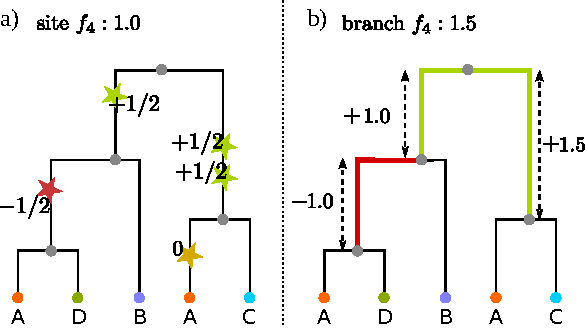
\includegraphics{figures/branch_site_diagram}
    \caption{
    Computing the $f_4(A,B;C,D)$ statistic on a tree.
    \textbf{(a)} Each mutation is given weight equal to $(p_A - p_B)(p_C - p_D)$,
    where $p_X$ is the proportion of the samples inheriting that mutation (colored stars) in set $X$
    (shown in labels at the bottom).
    Note that each of the mutations shown occurs at a distinct site, so there is no backmutation.
    \textbf{(b)} Each branch is assigned weight equal to the weight that would be assigned
    to any mutation falling in it (colored lined), and then the branch $f_4$ statistic
    is the sum over these weights, multiplied by the length of the branch
    (and the span of the tree, not depicted).
        \label{fig:branch_site_diagram}
    }
    \krt{This figure is not as helpful as fig 1. It takes a lot of fiddling to work out the values in each panel. Is it
    possible to fill it out as in fig 1, or is that just too much space?}
\end{figure}


This defines a statistic for a single window,
but in practice it is more useful to average branch statistics
over a region of the genome,
which we do by averaging the tree statistics over the region
with probabilities proportional to the trees' spans.
We write this with similar notation:
\begin{align}
    \branch(f, \iw)_{[c,d)}
    &=
    \frac{1}{d-c} \sum_{k=1}^{n(\treeseq)} \ell_k(c,d) \branch(f, \iw)_{T_k} ,
\end{align}
where $\ell_k(c,d)$ is the length of the region in $[c,d)$ that the tree $T_k$ covers
(i.e., if $T$ covers the half-open interval $[a_{k-1},a_k)$,
then $\ell_k(c,d) = \max(0, \min(d,a_k) - \max(c,a_{k-1}))$).

The \emph{polarised} version of a Branch statistic
is defined analogously to the Node and Site versions:
\begin{align} \label{eqn:branch_polarised}
    \text{(polarised)} \qquad
    \branchp(f, \iw)_T
    &=
    \sum_{u \in T} f(\nw_{T}(u)) ,
\end{align}
and $\branchp(f, \iw)_{[c,d)}$ is defined using $\branchp(f, \iw)_T$ as before.
However, the correspondence between the polarised statistics is less tight
than for the unpolarised ones.


\begin{example}[Mean TMRCA] \label{ex:branch_diversity}
    If we take $\iw$ and $f$ exactly as in the ``Nucleotide diversity'' example above,
    then $f(u)$ gives the probability that the branch ancestral to $u$
    lies on the path from one of two randomly chosen samples from $S$
    on the path up to their most recent common ancestor (MRCA).
    Therefore, $\branch(f, \iw)$
    gives the mean total distance in the tree between two samples from $S$,
    averaged across the sequence.
    This is twice the mean TMRCA if the samples are all from the same time.
\end{example}

\begin{example}[Phenotypic correlation with pedigree] \label{ex:branch_correlation}
    If we take $\iw$ and $f$ as in the ``Phenotypic correlations'' example above,
    what does $\branch(f, \iw)$ tell us?
    The statistic tells us the \emph{expected} correlation between phenotype and any mutations
    appearing on the tree, which is a summary of how much local relatedness
    aligns with similarity in phenotype.
\end{example}

The previous example might be used to leverage local relatedness
to improve the resolution of association studies.
Similar strategies were explored by \citet{zollner2005coalescent} and \citet{minichiello2006mapping}.

\begin{example}[Patterson's $f_4$] \label{ex:branch_f4}
    Suppose that the four subsets each consist of only a single sample.
    The summary function $f(x_1, x_2, x_3, x_4)$ for the $f_4$ statistic
    then assigns weight 1 to any branch that separates $x_1$ and $x_3$ from $x_2$ and $x_4$,
    and weight -1 to any branch that separates $x_1$ and $x_4$ from $x_2$ and $x_3$.
    The statistic $\branch(f, \iw)$ therefore
    gives the difference in average lengths of these two types of branch,
    averaged over choices of samples from the sample sets and averaged across the genome.
\end{example}


%%%%%%%%%%%%%%%%%%
\subsection*{General properties}

\plr{not sure if we need this section}

The statistics defined here are all \emph{additive} along the genome:
if we have computed a statistic in equal-size windows along a chromsome,
then the value of the statistic for the entire chromosome is equal to
the average of the values in those windows.
Some commonly-used statistics (e.g., $F_{ST}$ or Tajima's $D$)
are not additive, but are ratios of additive statistics, so can be easily computed in this way.
Multilocus statistics that measure linkage disequilibrium or haplotype lengths
do not fall in this category.
We have also defined site statistics to be additive across \emph{alleles},
to allow the definitions to apply to sites with more than two alleles.
This decision has some nice properties, but is not the only reasonable choice.

We also require that site statistics be computable from the genotype matrix
(i.e., without knowledge of the trees),
and, if the statistic is polarised, knowledge of the ancestral allele.
We often would also like our statistics to be unaffected by the addition of monomorphic sites,
which are usually omitted from genetic variation data.
To ensure this we have required that the summary function returns zero when give both zero weight
and the total weight: $f(0) = f(\tiw) = 0$.
This also makes branch and node statistics unchanged by portions of the tree that do not lie on a path
between any of the samples that have nonzero weight,
so that in particular,
\emph{simplification} of the tree sequence will not change the value of the statistic.
However, in practice this requirement can be relaxed.


%%%%%%%%%%%%%%%%%%
\section*{Duality of site and branch statistics}

Under a neutral, infinite-sites model of mutation with constant mutation rate across time,
the expected number of mutations per branch is proportional to its length.
This implies an isormorphism between ``site'' and ``branch'' statistics defined above,
which is discussed in more detail in \citet{ralph2019empirical}.
For instance, the site statistic of Example \ref{ex:site_diversity} (genetic diversity)
and the branch statistic of Example \ref{ex:branch_diversity} (mean TMRCA)
use the same summary function $f(x) = x(n-x)/n(n-1)$.
These are closely related because under an infinite-sites model of mutation,
two sequences differ at a site only if there has been a mutation somewhere on the branches going back
to their most recent common ancestor,
and so if mutations occur with constant rate,
the expected value of genetic diversity,
averaging over mutational noise give the tree sequence,
is equal to the mutation rate multiplied by the average distance between the two in the trees.

This relationship is true more generally.
In fact, for any region of the genome between $a$ and $b$,
with $\treeseq_{[a,b)}$ the trees spanning that interval,
\begin{align}
    \branch(f, \iw)_{[a,b)}
    =
    \E\left[ \site(f, \iw)_{[a,b)} \given \treeseq_{[a,b)} \right] ,
\end{align}
where the expected value averages over infinite-sites mutations with rate 1
(and so lengths are measured in units of expected numbers of mutations)
but leaves the genealogies fixed.
In other words, the Site statistic can be thought of an estimator of its corresponding Branch statistic,
which is itself a summary of local tree shapes.
Let's unpack the assumptions here: what exactly is the mutational model?
First, we are taking the mutation rate to be 1, i.e.,
the expected number of mutations that occur on a region of the genome of length $\ell$
over $t$ units of time is equal to $\ell t$.
This just amounts to a change of units --
for instance, if genome length is measured in nucleotides,
and the probability of mutation is $\mu$ per nucleotide and per generation,
then we are measuring times in units of $1/\mu$ generations.
Second, we are assuming that the probability of per-site mutation is low enough
that no two mutations occur at the same site
-- the fact that they do, occasionally, means that this is an approximation.
Third, we are assuming that mutation rates are constant through time and across the genome.
Of course, the statement remains true if we can measure distance along the genome and time
in a way that mutation rates are constant, but how these vary is generally unknown.

Note that the expected product of two site statistics,
$\E[\site(f, \iw) \site(g, \iw')]$
is not equal to the product of the two branch statistics, $\branch(f, \iw) \branch(g, \iw')$,
because they are not independent.
However, it is always possible to define a branch statistic that
gives the expected value of the product.
How to do this is described in \citet{ralph2019empirical}.

In this view,
site statistics are noisy approximations to the corresponding branch statistic
-- but, how noisy?
How big is the contribution of mutation to the overall sampling variance of a statistic?
Concretely the law of total variance lets us partition the variance of a site statistic
into the contributions of mutation and demographic noise:
\begin{align*}
    \var[\site(f, \iw)_{[a,b)}]
    &=
        \E\left[ \var\left[\site(f, \iw)_{[a,b)} \given \treeseq_{[a,b)}\right] \right]
        + \var\left[ \E\left[\site(f, \iw)_{[a,b)} \given \treeseq_{[a,b)}\right] \right] \\
    &=
        \E\left[ \var\left[\site(f, \iw)_{[a,b)} \given \treeseq_{[a,b)}\right] \right]
        + \var\left[ \branch(f, \iw)_{[a,b)} \right] .
\end{align*}
The first term, the variance of the statistic given the trees,
is the contribution to variance of mutation,
while the second term, the variance of the branch statistic,
is the contribution of demographic variation, including drift.
In the next section we examine this partitioning of variance using simulations.


%%%%%%%%%%%%%%%%%%%%%%%%%%%%%%%%%%%%%%%%
\subsection*{Branch statistics for population genetics}

We examined the contributions of mutation and demography to noise
in two simulations where population genetic (site) statistics
are important in making inferences:
detecting recent selective sweeps,
and detecting introgression.

Figure~\ref{fig:sweep_duality} shows windowed
diversity along the chromosome following a few selective sweeps.
The top two plots compare ``branch'' diversity -- i.e., as computed only with tree shape --
to ``site'' diversity computed from sequence generated by 20 independent assignments of mutations to the same tree sequence,
with mutation rates $10^{-9}$ and $10^{-8}$, respectively.
We see that as the mutation rate increases, the signal of decrease in diversity around swept loci becomes more clear,
and approaches ``branch'' diversity.
These were computed using the entire population of 1,000 individuals;
how does sampling variance contribute?
Not much, it turns out -- the bottom plot shows both site and branch diversity
computed from 20 nonoverlapping groups of 100 samples.
Neither site or branch diversity vary much between these samples,
implying that the subsample gives us a good estimate of the whole-population values of each.
However, as we see in the top figure,
whole-population site diversity is itself only a quite noisy estimator of branch diversity.
The same things are shown in Supplementary Figure \ref{sfig:sweep_duality_10K}
for a simulation with 10,000 individuals, which shows similar patterns.
Only the last of these plots is possible to directly observe in real data:
in the top two plots,
the spread of independent replicates of mutational noise (black lines)
about their expectation based on the tree sequence (red line)
is unobservable, although estimable.


\begin{figure}
    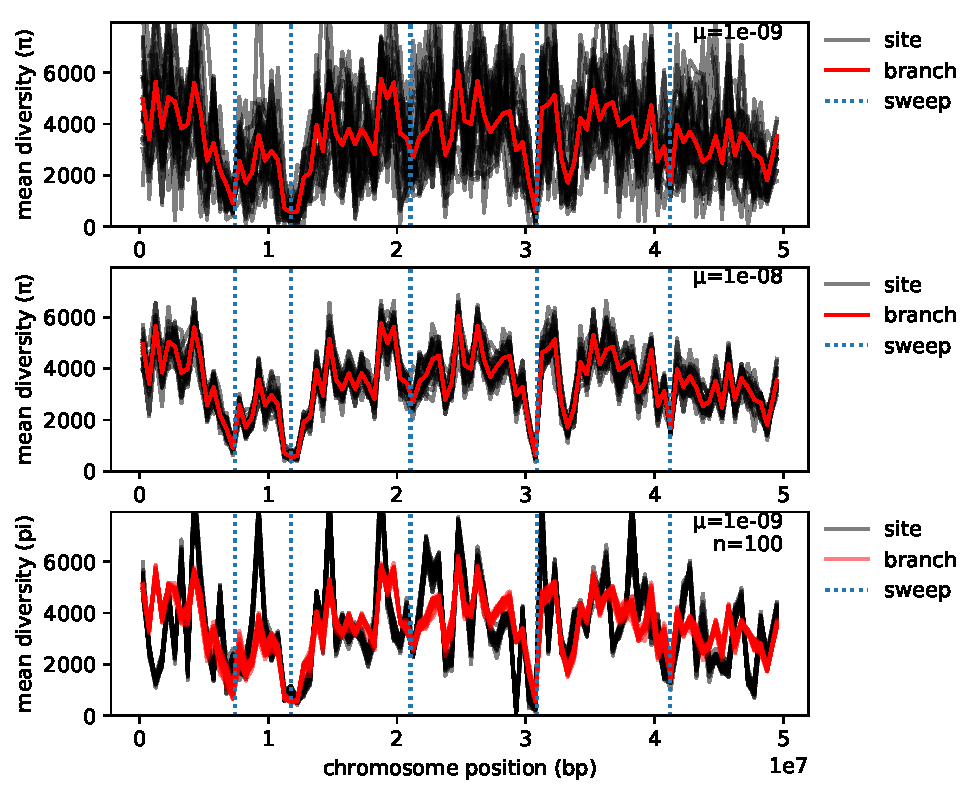
\includegraphics{{figures/swept.1000.999.1e-09.diversity}.pdf}
    \caption{
        Mean genetic diversity and time to most recent common ancestor
        in 500Kb windows along a 50Mb genome (0.5 Morgans) following several selective sweeps.
        In each case, ``site'' is mean genetic diversity (Tajima's $\pi$) divided by mutation rate,
        and ``branch'' is the corresponding branch statistic described above.
        The tree sequence was produced by simulating mutations under positive selection with mutation rate $10^{-12}$
        in a population of size 1000 for 400 generations using SLiM,
        followed by recapitation with $N_e=1000$.
        The selected alleles at the marked sites have selection coefficients between 0.08 and 0.25,
        and are at frequencies 96.8\%, 100\%, 16.25\%, 100\%, and 82.6\% in the final generation, respectively.
        All curves use the same tree sequence, including selected mutations,
        and with additional neutral mutations added.
        \textbf{(top)}
        Diversity within the entire population,
        computed using for mode ``site'' from 20 independent assignments of mutations to the same tree sequence with mutation rate $\mu = 10^{-9}$.
        \textbf{(middle)}
        As in the top panel, but with mutation rate $\mu=10^{-8}$,
        showing that as mutation rate increases, mode ``site'' (divided by $\mu$) converges to mode ``branch''.
        \textbf{(bottom)}
        ``Site'' and ``branch'' diversity within 20 disjoint samples of size 100 each,
        computed on a single tree sequence with mutation rate $\mu = 10^{-9}$.
        \label{fig:sweep_duality}
    }
\end{figure}


As another example, we simulated an ``admixture'' scenario:
a first population of size $N=1000$ splits into two of equal size,
then after $N$ generations, the second population splits,
after another $N$ generations, the third population splits again,
and for the final $N$ generations populations 2 and 3
have per-capita migration rates of $4/N$ to each other.
In this situation, a significantly negative $f_4(1,2;3,4)$ is expected,
which we indeed find, with a mean value of around -700.
Using various sample sizes, mutation rates, and window sizes, we then
calculated this $f_4$ statistic in windows along a 100Mb genome,
and show the standard deviation of both ``site'' and ``branch'' statistics across windows
in Figure \ref{fig:introf4}.
Since the genome is uniform (no selection or variation in recombination or mutation),
this standard deviation is a measure of noisiness.
As expected, site statistics are noisier than branch statistics,
by a factor that depends mostly on the ratio of mutation to recombination rates.
The results suggest that branch statistics would provide substantially better resolution
at small scales along the genome, especially if mutation rate is lower than recombination rate.
However, in practice imperfect estimation of the tree sequence
would introduce additional noise,
so it remains to be seen if the improvement could be made in practice.

\begin{figure}
    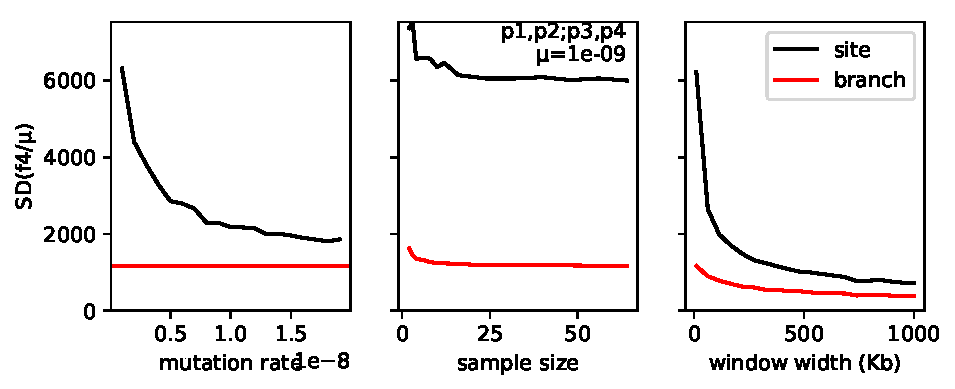
\includegraphics{{figures/intro/introgressed.1000.23.10000.1e-09.f4sd}.pdf}
    \caption{
        Standard deviation of site (black) and branch (red) $f_4(1,2;3,4)$
        in windows along a 100Mb genome, as a function of
        \textbf{(left)} mutation rate,
        \textbf{(middle)} sample size, and
        \textbf{(right)} window width.
        The recombination rate $10^{-8}$,
        and unless otherwise stated, the mutation rate was $10^{-9}$,
        the window width was 10Kb,
        and the entire population (1000 diploids in each of four populations) were used.
        \label{fig:introf4}
    }
\end{figure}


%%%%%%%%%%%%%%%%%%
\section*{Application to 1000 Genomes tree sequences}

We do not know the true genealogies underlying real data,
but recent methods are available to estimate them.
Above, we showed that branch and site statistics matched well in simulated data,
but these simulations made some simplifying assumptions, including constant mutation rates.
To evaluate the correspondence between site and branch statistics
in tree sequences inferred from real data,
we calculated mean sequence diversity along chromosome 20 from the 1000 Genomes dataset
in 1Mb windows separately in each of the five continental groupings,
calculated using the site statistic described in Example~\ref{ex:site_diversity},
and compared this to the dual branch statistic (of Example~\ref{ex:branch_diversity})
as calculated from three inferred tree sequences:
by \tsinfer{} \citep{kelleher2019inferring}, which only aims to estimate tree topologies,
not well-calibrated node times,
(2) by GEVA \citep{albers2019dating}, which aims to calibrate the node times reported by \tsinfer,
and (3) by Relate \citep{speidel2019method}, an independently developed method.
All calculations were done only using the portions of the chromosome
passing the 1000 Genomes Phase 1 ``strict'' mask for sequencing accessibility.
% from ftp://ftp.1000genomes.ebi.ac.uk/vol1/ftp/phase1/analysis_results/supporting/accessible_genome_masks/README.20120515_phase1_pop_gen_mask
Separate curves for each of the 26 sampling locations are shown in Supplemental Figure \ref{fig:chr20_full}.

The comparisons are shown in Figure~\ref{fig:chr20}.
Of these methods, branch diversity from \tsinfer{} shows the worst agreement with site diversity,
which is unsurprising as \tsinfer{} uses allele frequency as a proxy for age.
The two methods that infer node times differ substantially,
with Relate showing a significantly tighter agreement than GEVA.
Does this mean that Relate is doing a better job at inferring the tree sequence than \tsinfer/GEVA?
Answering this question requires a deeper understanding of the processes that shape
genetic diversity along the genome.

\begin{figure}
    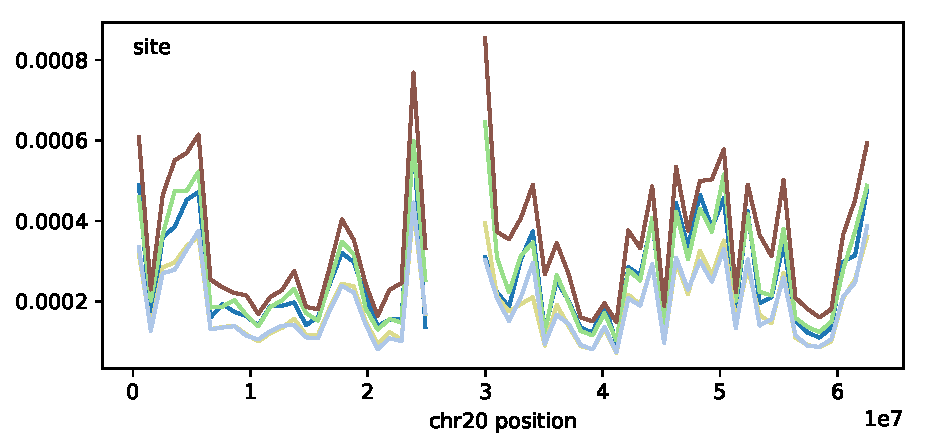
\includegraphics[width=0.5\textwidth]{{figures/1kg/relate_chr20.site.1000000.region.diversity}.pdf}
    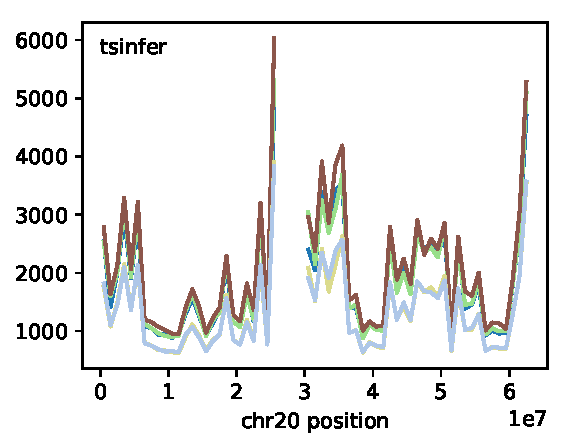
\includegraphics[width=0.5\textwidth]{{figures/1kg/1kg_chr20.branch.1000000.region.diversity}.pdf}
    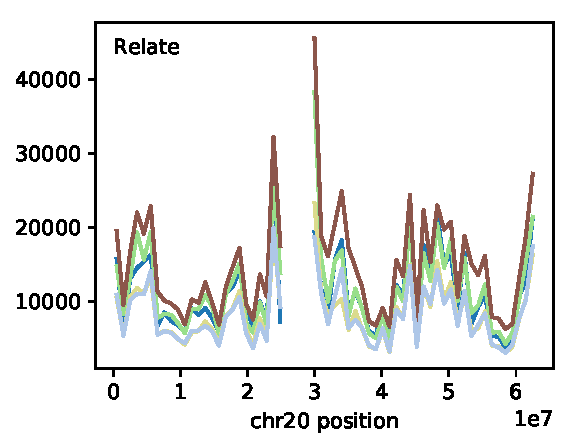
\includegraphics[width=0.5\textwidth]{{figures/1kg/relate_chr20.branch.1000000.region.diversity}.pdf}
    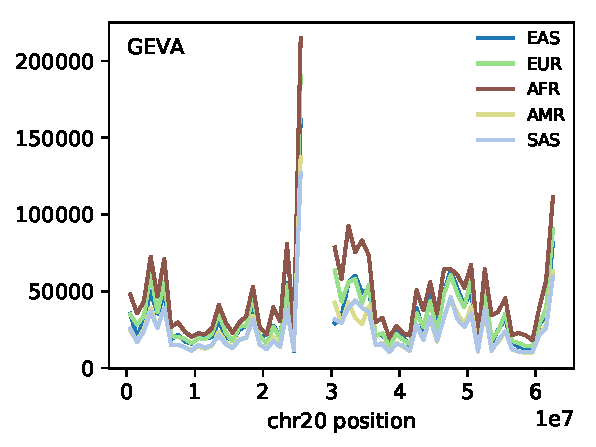
\includegraphics[width=0.5\textwidth]{{figures/1kg/tgp_geva_chr20.branch.1000000.region.diversity}.pdf}
    \caption{
        \textbf{(top left)} Mean sequence diversity
        in 1Mb windows along human chromosome 20 of the 1000 Genomes Project,
        and the dual branch statistic as calculated from tree sequences inferred by
        \textbf{(top right)} \tsinfer,
        \textbf{(bottom left)} Relate, and
        \textbf{(bottom right)} GEVA/\tsinfer.
        Separate curves are plotted for each sampling location.
        \label{fig:chr20}
    }
\end{figure}

In practice, we do not expect branch and site diversity to agree exactly,
because of local differences in mutation rate and intensities of selected mutations.
For instance, regions in which a high proportion of potential mutations are deleterious
are expected to have a lower diversity for two reasons:
first, the deleterious mutations themselves are less likely to be found,
and second, the indirect effect of deleterious mutations on nearby sites reduces typical tree height
and thus diversity at even neutral, linked sites \citep{hudson1994levels,charlesworth1997effects}.
The first effect would cause site and branch statistics to differ,
because it effectively reduces the mutation rate in the region
and violates the assumption of independence of mutations given the trees.
However, the second effect does \emph{not} affect the correspondence between site and branch statistics,
since it is mediated by tree shape.
However, it is generally unknown how much mutation rate varies along the genome
\citep[but see][]{supek2015differential}
or how dense are targets of selection \citep{leffler2012revisiting}.
For this reason, it is very interesting to see how close a correspondence between site and branch
statistics it is \emph{possible} to obtain --
it is tempting to say that the best tree sequence would obtain
as tight a match between site and branch statistics as possible,
with remaining variation explained by direct selection and/or mutation rate variation.


%%%%%%%%%%%%%%%%%%%%%
\subsection*{Time stratification of statistics}

Thus far we have examined how statistics vary along the genome,
but a tree sequence allows us access to another dimension: time.
Next, we examine the \emph{time} distribution of admixture signal
in the tree sequence inferred by \tsinfer/GEVA.
The branch $f_4(A, B; C, D)$ statistic for four sample sets $A$, $B$, $C$, and $D$
is the sum of $(p_A - p_B)(p_C - p_D)$ across branches, multiplied by span and height,
where $p_X$ is the proportion of samples in sample set $X$ that inherit from that node.
A branch with a large value is expected to contribute a large amount to the Site $f_4$,
which is calculated from genotyping data
and is used to infer historical connections between populations.
To visualize the time signature, we assigned the contribution of each branch
to its terminal node,
and then summed these values across all nodes in 50 logarithmically-spaced bins by time.
We then normalised these to sum to 1 by dividing by the total Branch $f_4$ value.

The four-tuple of sample sets for the first two statistics (PUR,TSI;GWD,JPT and ASW,CEU;MSL,CHB)
are from similar regions of the world,
and show almost identical time signatures,
even though the second set of sample sets has a value of $f_4$ nearly eight times higher.
The second two statistics (IBS,GBR;FIN,JPT and TSI,CEU;FIN,CHB) are also comparable,
and also show similar signals to each other.
These curves are noisier, because the $f_4$ values are much smaller.
For all four comparisons, the largest contribution to $f_4$ comes from
ancestors living tens of thousands of generations ago.
\plr{WHAT IS THE TIME UNIT?}
This is surprising, because $f_4$ is expected to deviate from zero due to asymmetries in tree topology
during recent history (e.g., more branches ancestral to ASW and MSL than CEU and MSL).
Furthermore, we expected the different sample sets to have much more distinct time signatures.
The shared, ancient time signatures may be because nonzero $f_4$ statistics
are due to differentially sorting ancestral variation,
or inacurracies in tree sequence inference.
It is tempting but propably unwarranted to attribute the
large downward spike between 2000 and 3000 generations in the TSI,CEU;FIN,CHB comparison
to a historical connection between the ancestors of CEU and the Finnish not shared by the Tuscans
during that time period.
Making rigorous conclusions from this sort of visualization
will require substantial validation work
to understand the various sources of bias and uncertainty.


\begin{figure}
    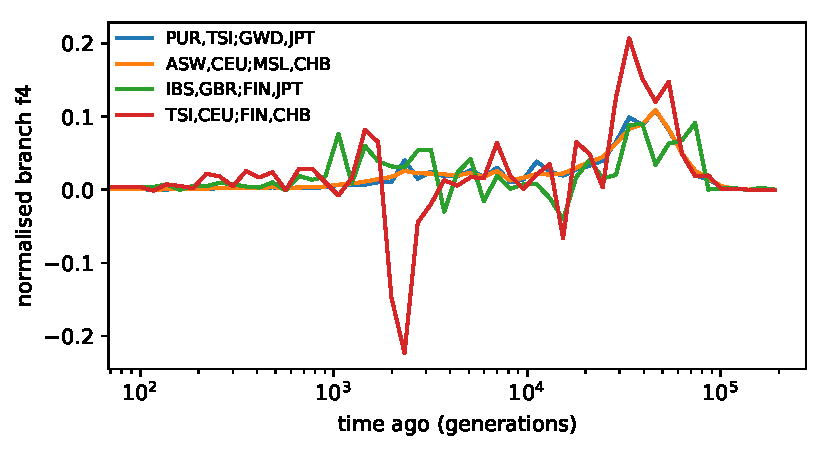
\includegraphics{{figures/1kg/tgp_geva_chr20.node.time.f4}.pdf}
    \caption{
        Time distribution of signal for four $f_4$ statistics
        in the tree sequence for chromosome 20 inferred from 1000 genomes data by GEVA.
        The branch $f_4$ statistics for these four are:
        PUR,TSI;GWD,JPT: 1603,
        ASW,CEU;MSL,CHB: 12587,
        IBS,GBR;FIN,JPT: -129, and
        TSI,CEU;FIN,CHB: -96.
        Population codes are
        `PUR': Puerto Ricans from Puerto Rico;
        `TSI': Toscani in Italia;
        `GWD': Gambian in Western Divisions in the Gambia;
        `JPT': Japanese in Tokyo, Japan;
        `ASW': Americans of African Ancestry in SW USA;
        `CEU': Utah Residents (CEPH) with Northern and Western European Ancestry,
        `MSL': Mende in Sierra Leone;
        `CHB': Han Chinese in Beijing, China;
        `IBS': Iberian Population in Spain;
        `GBR': British in England and Scotland;
        and `FIN': Finnish in Finland.
        \label{fig:node_f4}
    }
\end{figure}



%%%%%%%%%%%%%%%%%%
\section*{Efficient algorithms and implementation}

%%%%%%%%%%%%%%%%%%%%%
\subsection*{Algorithms}
In this section we describe and analyse the algorithm used
to compute branch length statistics. This is a generalization
of the algorithm used to maintain the number of samples from a
given set that derive from each node in a tree
sequence \cite[Algorithm L]{kelleher2016efficient}. The central
problem which is shared across site, branch and node statistics
is to efficiently maintain the ``state'' $x_u$ (where $x_u$ is the
sum of the weights for all samples descending
from, and including, node $u$; see Figure~\ref{fig:divergence_diagram}).
As we move along the sequence, the trees change when branches are inserted and removed.
By carefully ordering these insertions and removals,
we ensure that this state can be correctly maintained
using only small adjustments for each tree.
Computing the statistics is then a straightforward matter of applying the summary function $f$
to the node states and aggregating the results appropiately for the
particular statistics mode and windowing options.

Formally, we represent a tree sequence using a set of tables~\citep{kelleher2018efficient}.
Each node describes a particular haplotype (i.e., one of the two genomes of a diploid individual),
and details about these haplotypes are stored in a node table, $\Nt$.
The row $\Nt[u]$ contains all information about the node $u$, and rows
are indexed from zero such that $0 \leq u < |\Nt|$.
In particular, the birth time for $u$ is given by $\Nt[u]\prop{time}$.
Information about how nodes relate to each
other along the genome is encoded in an edge table, $\Et$.
For a given row $j$, $\Et[j]\prop{child}$ and $\Et[j]\prop{parent}$
define a parent-child relationship between two nodes in a set of
contiguous trees along the genome. $\Et[j]\prop{left}$ then denotes
the left-most (inclusive) and $\Et[j]\prop{right}$ the right-most
(exclusive) genome coordinates over which this branch exists.
The order in which edges are inserted and removed is determined
by the ``index vectors'' $\indexin$ and $\indexout$~\citep{kelleher2016efficient}.
The ``edge insertion'' vector $\indexin$ gives the ordering of edges
sorted by left endpoint, and among edges with the same left endpoint,
sorted so that edges closer to the root appear later.
The ``edge removal'' vector $\indexout$ is similar, except gives the ordering of edges
by right endpoint and with edges closer to the root appearing sooner.
\plr{is that right?}
As we move along the tree sequence, the topology of the current tree is recorded in the
``parent vector'' $\pi$: the parent of each node $u$ is the node $\pi_u$,
with $\pi_u = -1$ if $u$ is a root.
Similarly, we maintain the branch length vector $\beta$ by setting
$\beta_u = \Nt[\pi_u]\prop{time} - \Nt[u]\prop{time}$ and
$\beta_u = 0$ if $u$ is a root. As evaluating the summary function
$f$ is an expensive operation, we also maintain the vector $F$
such that $F_u = f(x_u)$. For notational simplicity here we assume
that weights and summary functions are scalars, but the extension to
vectors is trivial. We also assume that we are computing the statistic
across the full span of the tree sequence; the extension to multiple windows is routine.
See below for a description of the steps in words,
and \autoref{fig:algorithm_example} for an example of the internal state of the algorithm.

\begin{taocpalg}{B}{General branch statistics}
{Given a list of $n$ sample nodes $S$, corresponding weights $w$ and
summary function $f: \R \rightarrow \R$
compute the span-normalised statistic $\sigma$
over a tree sequence with sequence length $L$
defined by the node and edge tables $\Nt$ and $\Et$. We assume
that the index vectors $\indexin$ and $\indexout$ have been precomputed.
}

\algstep{B1.}{Initialisation.}{
    For $0 \leq u < |\Et|$ set $\beta_u \leftarrow x_u
    \leftarrow F_u \leftarrow 0$ and $\pi_u \leftarrow -1$.
    Then, for $0 \leq j < n$ set $u \leftarrow S_j$,
    $x_u \leftarrow w_j$ and $F_u \leftarrow f(x_j)$. Finally,
    set $s \leftarrow \sigma \leftarrow j \leftarrow k \leftarrow t_l \leftarrow 0$.
}

\algstep{B2.}{Terminate.}{If $j \geq |\Et|$ or $t_l \geq L$,
    return $\sigma / L$ and terminate.
}

\algstep{B3.}{Edge removal loop.}{If $k \geq |\Et|$ or $t_l \neq
    \Et[\indexout_k]\prop{right}$ go to \algref{B6}.}

\algstep{B4.}{Remove edge.}{Set
    $u \leftarrow \Et[\indexout_k]\prop{child}$,
    $v \leftarrow \Et[\indexout_k]\prop{parent}$ and $k \leftarrow k + 1$.
    Then set $s \leftarrow s - \beta_u F_u$, $\pi_u \leftarrow -1$
    and $\beta_u \leftarrow 0$.
}

\algstep{B5.}{Propagate loss.}{While $v \neq -1$, set
    $s \leftarrow s - \beta_v F_v$, $x_v \leftarrow x_v - x_u$,
    $F_v \leftarrow f(x_v)$, $s \leftarrow s + \beta_v F_v$
    and $v \leftarrow \pi_v$. Afterwards, go to \algref{B3}.
}

\algstep{B6.}{Edge insertion loop.}{If $j \geq |\Et|$ or $t_l \neq
    \Et[\indexin_j]\prop{left}$ go to \algref{B9}.}

\algstep{B7.}{Insert edge.}{Set
    $u \leftarrow \Et[\indexin_j]\prop{child}$,
    $v \leftarrow \Et[\indexin_j]\prop{parent}$ and $j \leftarrow j + 1$.
    Then set $\pi_u \leftarrow v$,
    $\beta_u \leftarrow \Nt[v]\prop{time} - \Nt[u]\prop{time}$ and
    $s \leftarrow s + \beta_u F_u$.
}

\algstep{B8.}{Propagate gain.}{While $v \neq -1$, set
    $s \leftarrow s - \beta_v F_v$, $x_v \leftarrow x_v + x_u$,
    $F_v \leftarrow f(x_v)$, $s \leftarrow s + \beta_v F_v$
    and $v \leftarrow \pi_v$. Afterwards, go to \algref{B6}.
}

\algstep{B9.}{Tree loop tail.}{Set $t_r \leftarrow L$.
    If $j < |\Et|$ set $t_r \leftarrow \min(t_r, \Et[\indexin_j]\prop{left})$.
    Then, if $k < |\Et|$ set $t_r \leftarrow \min(t_r, \Et[\indexout_k]\prop{right})$
    Finally, set $\sigma \leftarrow \sigma + (t_r - t_l)s$,  $t_l \leftarrow t_r$
    and go to \algref{B2}.
}

\end{taocpalg}

Algorithm \algref{B} begins by setting the initial state for $\pi$, $\beta$,
$x$ and $F$ for each node in the tree sequence, and then sets the values
of $x_u$ and $F_u$ for each of the samples $u$ in $S$.
(The initial state is the ``empty forest'', where no nodes are connected to any others.)
Afterwards, we set our ``running sum'' $s$ and output statistic $\sigma$ to zero, along
with the ``tree left'' variable $t_l$. The $j$ and $k$ variables are
used to keep track of our position in the edge insertion and edge
removal indexes, respectively. After completing initialisation in
\algref{B1}, we enter the main tree loop in \algref{B2} which is
run once for each tree in the sequence. As we are processing each
tree, we keep track of the edges that need to be processed with
the $t_l$ variable, which stores the left-most genome coordinate
in the current tree. The first thing we do for a new tree is to
remove any edges that were in the previous tree are not in the
current tree. These must be the edges in which the right coordinate
is equal to $t_l$, and so \algref{B3} loops over these edges using
the edge removal index $\indexout$. Step \algref{B4} then removes
the branch $u \mapsto v$ corresponding to a single edge, by
subtracting its contribution to the running sum $s$, setting the parent of
$u$ to $-1$ and its branch length to $0$. As shown in
Figure~\ref{fig:algorithm_example}B, removing an edge will result
in the subtree rooted at $u$ become disconnected from the rest of the
tree. Step \algref{B5} ensures that the state of the rest of the tree
is correctly maintained by propagating the loss of the state $x_u$
up the tree from $v$. Thus, for each direct ancestor $v$ that was a
direct ancestor of $u$ in the previous tree, we first subtract
its contribution from the running sum $s$ and remove the contribution
of $x_u$ from its state. Since the state of $v$ has changed, we must
recompute the value of our summary cache $F_v$, and then finally
add the new contribution of $v$ to $s$. (For example, note the changes in $x$
and $F$ for nodes 7 and 8 in Figure~\ref{fig:algorithm_example}B.)

Once all of the edges with right coordinate equal to $t_l$ have been removed in
steps \algref{B3--B5}, we then insert edges that start in the current tree
(i.e., with left coordinate $t_l$) in steps \algref{B6--B8}. We update the
state to account for the new branch $u \mapsto v$ by setting the parent of
$u$ to $v$, computing the branch length of $u$ and adding the new contribution
of $u$ to $s$ in \algref{B7}. Then, as adding a new edge can connect the
subtree rooted at $u$ to the larger tree at $v$, we propagate the gain of $x_u$
up the tree in step \algref{B8} (note the symmetry with step \algref{B5}).
Finally, once we have removed and inserted all of the relevant edges, we are
ready to add the contribution of the current tree to the overall statistic,
$\sigma$ and move on to the next tree in step \algref{B9}. To do this, we first
compute the right-hand coordinate of the tree $t_r$ (a process slightly
complicated by the possible presence of ``gaps'' in the tree sequence, spanned
by no edges). Then, we add the running sum $s$ weighted by the span of the
current tree $t_r - t_l$ to $\sigma$, and return to \algref{B2} to process the
next tree. If we have reached the end of the sequence, we then divide $\sigma$
by the sequence length to renormalise and exit.

To analyse Algorithm~\algref{B} we will assume that the tree sequence has
been simulated under the standard coalescent with a sample of size
$n$ and population scaled recombination rate $\rho = 4 N_e r$,
where $r$ is the mean number of recombinations per chromosome per unit of time.
Under these conditions, there are $O(n + \rho \ln n)$ edges in the tree sequence
\citep{kelleher2016efficient}.  Clearly, each edge is examined
exactly once in steps \algref{B6} and \algref{B7} in order to create
the trees, and at most once in steps \algref{B3} and \algref{B4} (we do
not remove the edges for the final tree). Additionally, each edge that
we insert or remove after the initial building of the tree
may incur the cost of traversing up the tree as
far as the root in steps \algref{B5} and \algref{B8}.
As coalescent genealogies are asymptotically
balanced \citep{li2013coalescent}, the expected number of nodes
on the path to root is $\log_2 n$.
Therefore, the overall running time
of Algorithms~\algref{B} is of order $n + \rho \log(n) \log_2(n)$, which is
\[
    O\left(n + \rho \log(n)^2 \right)
\]
Computing a site statistic will have the same complexity,
as the same internal state is maintained,
and the number of segregating sites is proportional to the number of edges
(with constant equal to the ratio of mutation to recombination rate).
The asymptotic analysis here assumes that we traverse upwards to root
for each edge, but this is not the case. Edges are removed in
oldest-first order, guaranteeing that the deepest node any subtree being
modified is processed first. Therefore, this subtree will be disconnected from the
main tree, ensuring that we traverse upwards all the way to root only once.
Similarly, edges are inserted in youngest-first order, ensuring that subtrees are only
reconnected to the main tree when they are fully built.

\begin{figure}
    % Run the script illustrate_algorithm.py to generate these pdfs and
    % the latex tables below.
    \begin{center}
    \begin{tabular}{ccc}
    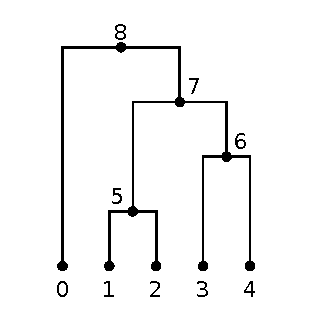
\includegraphics[width=4cm]{figures/tree_0_init.pdf} & &
    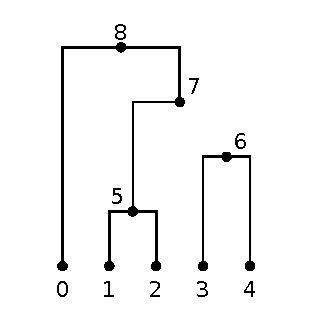
\includegraphics[width=4cm]{figures/tree_0_out_0.pdf}
    \\

    \begin{tabular}{c|cccc}
    & $\pi$ & $\beta$ & $x$ & $F$\\
    \hline
    0 & 8 & 4.0 & 1.0 & 0.2\\
    1 & 5 & 1.0 & 1.0 & 0.2\\
    2 & 5 & 1.0 & 1.0 & 0.2\\
    3 & 6 & 2.0 & 1.0 & 0.2\\
    4 & 6 & 2.0 & 1.0 & 0.2\\
    5 & 7 & 2.0 & 2.0 & 0.3\\
    6 & 7 & 1.0 & 2.0 & 0.3\\
    7 & 8 & 1.0 & 4.0 & 0.2\\
    8 & -1 & 0.0 & 5.0 & 0.0\\
    \end{tabular}
    & &
    \begin{tabular}{c|cccc}
    & $\pi$ & $\beta$ & $x$ & $F$\\
    \hline
    0 & 8 & 4.0 & 1.0 & 0.2\\
    1 & 5 & 1.0 & 1.0 & 0.2\\
    2 & 5 & 1.0 & 1.0 & 0.2\\
    3 & 6 & 2.0 & 1.0 & 0.2\\
    4 & 6 & 2.0 & 1.0 & 0.2\\
    5 & 7 & 2.0 & 2.0 & 0.3\\
    6 & -1 & 0.0 & 2.0 & 0.3\\
    7 & 8 & 1.0 & 2.0 & 0.3\\
    8 & -1 & 0.0 & 3.0 & 0.3\\
    \end{tabular}
    \\
    (A) && (B)
    \end{tabular}
    \end{center}

    \caption{
    Illustration of the internal state for algorithm B for $\iw = \bone_S$ and
    $f(x) = x(5 - x) / 20$ as in Example~\ref{ex:site_diversity}. (A)
    Immediately before we remove the edge joining 6 to 7 and (B) immediately after.
    See the text for descriptions of the arrays encoding the state.
    \jk{TODO: the value of $s$ would be helpful here too.}
    \label{fig:algorithm_example}}
\end{figure}

%%%%%%%%%%%%%%%%%%%%%
\subsection*{Speed}

\krt{need to sort out the big-O issue here}
We used coalescent simulations to compare the performance of calculating Tajima's \citeyearpar{Tajima1989-de} $D$
statistic from tree sequences to calculating it from integer matrices containing genotypes at all variable positions.
\autoref{fig:stats_performance} shows that the tree sequence methods implemented in \texttt{tskit} processes variant data
substantially faster than matrix-based approaches once the sample size is above $n \approx 500$ haploids --
three times faster for one thousand haplotypes,
growing to nearly three orders of magnitude faster for one million haplotypes.
The expected number of mutations for each replicate is $10^4 \times \sum_{i=1}^{n-1}\frac{1}{i}$, and thus ranges from
$\approx 32,000$ to $\approx 138,000$ \citep{Watterson1975-ej}.
\autoref{fig:stats_performance} only considers the time required to calculate the statistic,
and does not include the time required to build the genotype matrix, nor the memory required to store it.
For the largest samples size of $n=10^6$,
the matrix is approximately 200 gigabytes, and thus not practical on many systems.
The largest tree sequence simulated required less than one gigabyte of memory.

\autoref{fig:stats_performance} shows that \texttt{tskit} requires more time per variant once the sample size is larger
than $n \approx 10^4$.
This occurs because for large sample sizes,
the $O(n)$ complexity of building the first tree dominates the run time,
a cost that is amortized in longer genomes where more recombination leads to more trees.


\begin{figure}
    \centering
    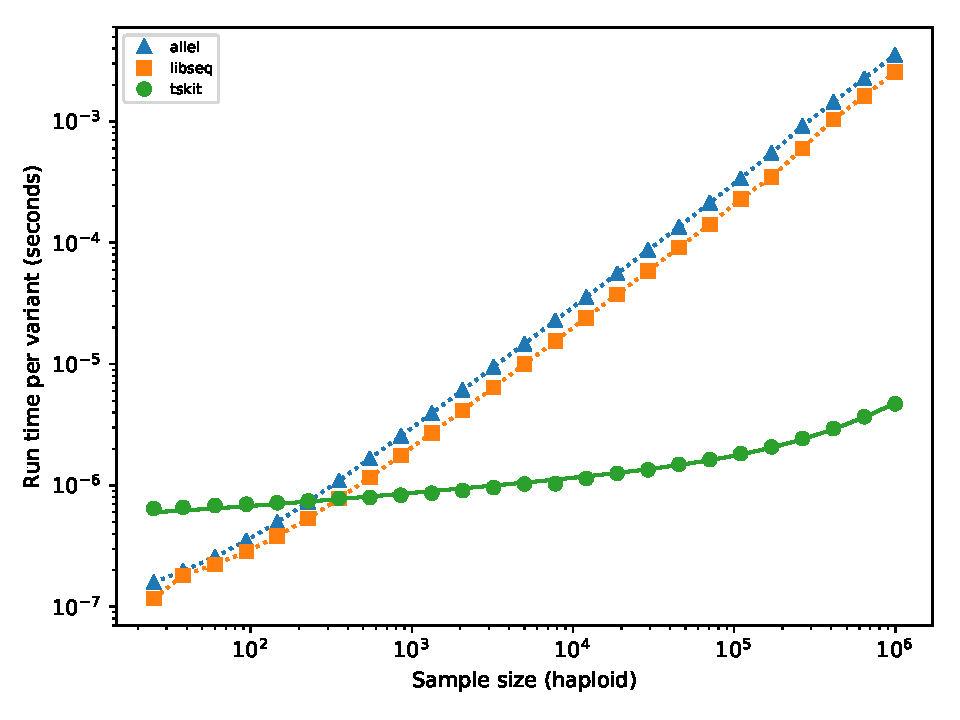
\includegraphics{tskit_stat_benchmarks/benchmarks_without_copy_longer_genome.pdf}
    \caption{Comparison of time required to compute site statistics
        between matrix and tree based methods. For each sample size, a single replicate
        was obtained using \texttt{msprime} with scaled neutral mutation rate $\theta = 4N_e\mu$ and
        scaled recombination rate $\rho = 4N_er$ both equal to $10^4$ and $N_e = 10^4$,
        where $\mu$ and $\rho$ are the total mutation and recombination rate across the simulated region
        per generation, respectively.
        For each replicate, Tajima's $D$
        \citep{Tajima1989-de} statistic was calculated using \tskit, \texttt{libsequence}
        \citep{Thornton2003-wj}, and \texttt{scikit-allel} \citep{miles2017scikit}.
        The solid green line shows the result of fitting the timing data to a model based on the expected complexity of the
        algorithm used by \texttt{tskit}. \krt{need to revisit the correctness of this}
        \label{fig:stats_performance}
    }
\end{figure}




%%%%%%%%%%%%%%%%%%%%%%%
\section*{Discussion}

% overview: general definition that is mostly functions of jAFS but includes others
In this paper, we have described a general framework for summarising genetic variation
and the underlying genealogies
that encompasses many standard population genetic statistics
and makes it easy to explore more.
Many of these statistics are functions of the joint allele frequency spectrum,
but the framework is more general,
and can be used to quantify associations between genotypes and phenotypes.
This generality was motivated in part by laziness --
adding new statistics is now almost as easy as working out the appropriate summary function --
but also makes it easy to computationally explore new classes of statistics.
The range of statistics available to describe variation in a single exchangeable sample
(i.e., a single population) are well-understood,
but there are much larger and less well-explored classes of statistics
describing genetic variation between many populations
or across geographical space.

% speed/efficiency: big data sets; large simulations
The most obvious application of these methods on current practice
is to improve efficiency of existing pipelines,
as tree sequences allow storage and processing of large genomic data sets
with orders of magnitude less space and time than most other methods.
All statistics described here (and more) are implemented
in the fast, rigorously tested python library \tskit{}
that also provides tools for working with tree sequences.
The largest efficiency gains are found for very large sample sizes
only likely to be available in real data sets for humans in the near future,
but the ability to analyze millions of whole genomes
is useful for understanding evolutionary simulations of any species
\citep[see][for a recent example]{galloway2019stickleback}.


% duality: site stats ~ branch stat, but conversely branch more accurate version of site
%  maybe analogous to imputation
We hope a more broadly interesting and useful aspect of this paper
is a more in-depth look at the correspondence between statistics calculated with genome sequence
and properties of the underlying genealogies, i.e.,
the duality between Site and Branch statistics under the infinite-sites model.
This general correspondence is well-known,
but the common framework implemented here makes it easy to translate between the two.
One way to use this translation is to answer:
what aspect of tree shape is this population genetics statistic summarising?
This can help when interpreting results, especially if reality may not fit an idealised model
of separate populations.
However, methods to infer tree sequences from real data
make it now possible to work in the other direction:
instead of calculating (Site) statistics from the genotype matrix,
we can calculate precisely analogous (Branch) statistics from the trees themselves,
thus hopefully bypassing the extra layer of noise induced by mutation.
How well this works will depend on the ability of inference methods
to infer the true tree sequence.
This might plausibly produce less noisy estimates because tree sequence inference
essentially uses the signal from nearby patterns of variation
to interpret relationships at a given site,
thus tranforming the simple binary split induced by a SNP
into a much richer source of information at every variant site.
Furthermore,
if tree sequence inference can be made insensitive to local variation in mutation rate,
calculation of branch statistics would provide a summary method
that is not affected by this potentially important confounding factor.

% visualization and time decomposition adding a new dimension
Genomic data are naturally distributed along two axes: along the genome, and across geography.
The tree sequence extends this to a third axis: time.
A great many methods in population genetics aim to describe aspects of history,
and accurate (or at least unbiased) tree sequence inference
may shift the focus of these problems from inference to descriptive analysis.
In this paper, we have made an exploratory foray in this direction,
by describing the time of origin of the ``admixture'' signal of nonzero $f_4$
between several subsets of the 1000 Genomes dataset,
in several inferred tree sequences.
It is not yet clear whether these time profiles tell us more about history
or about biases of the the inference methods,
but either result would be useful.

% moving past a few summaries in discrete groups to a genome/time/space view of relatedness
The historical toolbox of population genetics
is still mostly composed of statistics designed for analysis of a handful of loci
in a small number of discrete, mostly separated populations.
Both our data and our understanding of the world have moved beyond this.
We hope that the tools we develop here will help make it possible
to visualize and analyze genetic variation and genealogical realtedness
along the genome, across space, and through time.
\plr{okay rein me in here}


\paragraph{Future work}
In this paper,
we have considered only so-called additive, single site statistics.
Extensions to statistics involving the pairwise joint distribution of genotypes across sites
\citep[as used by][]{hudson2001twolocus},
such as linkage disequlibrium are planned for future work.
Haplotype-based statistics may require different classes of algorithms.




%%%%%%%%%%%%%%%%%%%%%%%
\subsection*{Acknowledgements}
Thanks to Graham Coop, Andrew Kern, Nick Patterson, and Kelley Harris for useful suggestions
and to Wilder Wohns and Leo Speidel for providing inferred tree sequences.


\bibliography{references}

\clearpage
\appendix
\setcounter{table}{0}
\renewcommand{\thetable}{S\arabic{table}}
\setcounter{figure}{0}
\renewcommand{\thefigure}{S\arabic{figure}}




%%%%%%%%%%%
\appendix

\section{Linear regression}
\label{apx:regression}

Let $h$ be a trait, $Z$ be a matrix of covariates, and $g$ be a vector denoting inheritance
(so, with $n$ samples, $h$ and $g$ are both $n$-vectors and $Z$ is an $n \times k$ matrix).
We would like to find the coefficient of $g$ in the linear regression of $h$ against $g$ and $Z$,
without doing full multivariate regression for every new $g$,
using the fact that $Z$ is always the same.
Suppose that $Z^T Z = I$ and that the vector of all ones is in the span of the columns of $Z$,
although in the implementation we post-process $Z$ to make this the case.
Then, let $a$ be the number and $b$ be the $k$-vector satisfying
\begin{align*}
    a, b = \text{argmin}\left\{ \sum_i \left( w_i - a g_i - \sum_j Z_{ij} b_j \right)^2 \right\}
\end{align*}
Writing this in block matrix notation, $a$ and $b$ minimise
\begin{align*}
    \left\|
        \left[ \begin{array}{@{}c@{}} h \end{array}\right]
            -
        \left[ \begin{array}{@{}c|c@{}} g & Z \end{array} \right]
            \left[ \begin{array}{@{}c@{}} a \\ \hline b \end{array} \right]
    \right\|^2 .
\end{align*}


Letting $B = [g | Z]$, the solution to this is
\begin{align*}
    \left[\begin{array}{@{}c@{}}a\\\hline b\end{array}\right]
        = (B^T B)^{-1} B^T h ,
\end{align*}
as long as $B^T B$ is invertible (which we assume to be the case).
Let $m = g^T g$ be the number of alleles in the sample coded 1,
let $u = g^T Z$ be the vector giving sums of the covariates of all samples carrying the allele,
and
\begin{align*}
    \alpha
    &=
        (g^T g - g^T Z (Z^T Z)^{-1} Z^T g) \\
    &=
        m - \sum_j u_j^2 .
\end{align*}
$\alpha$ is the norm of the component of $g$ not in the subspace spanned by the columns of $Z$,
so if $\alpha = 0$ then we want to return $a=0$.

Otherwise, by the inversion formula for a block two-by-two matrix,
since we have assumed that that $Z^T Z = I$,
\begin{align*}
    (B^T B)^{-1}
    &=
    \left[
        \begin{array}{@{}cc@{}}
            m & u \\
            u^T & I
        \end{array}
    \right]^{-1} \\
    &=
    \left[
        \begin{array}{@{}cc@{}}
            1/\alpha
            &
            - u / \alpha
            \\
            - u^T / \alpha
            &
            m \left(m I - u u^T \right)^{-1}
        \end{array}
    \right] .
\end{align*}
Now, the regression coefficient we seek is,
with $h_g = g^T h$,
\begin{align*}
    a
    &=
    \frac{1}{\alpha} \left(
        h_g - u Z^T h
    \right) .
\end{align*}

To compute this in the framework above,
first add a column of 1s to the covariates $Z$,
then decorrelate the resulting matrix, so that now $Z^T Z = I$.
Then, put this normalised version of $Z$
into the first $k$ columns of the weight matrix (so that $w_j(u) = Z_{uj}$),
set the $(k+1)^\text{st}$ column to the trait (so that $w_{k+1}(u) = w_u$),
and the final column to all $1$s (so $w_{k+2}(u) = 1$).
Also let $Z^T h = v$ be precomputed.
Then the sum of the traits of samples with the focal genotype is $h_g = x_{k+1}$,
and the allele count is $m = x_{k+2}$,
so that
\begin{align*}
    a
    &=
    \frac{
        h_g - \sum_{j=1}^k x_j v_j
    }{
        m - \sum_{j=1}^k x_j^2 } .
\end{align*}

In practice we square this and divide by two,
so that for biallelic loci the two alleles contribute an equal amount.
For loci with more than two alleles,
it would be more satisfying to return the proportion of variance in the trait
that is explained by \emph{all} of the alleles;
however, this would be more involved
(it would entail inversion of a $3 \times 3$ matrix for each locus).

% # NUMERICAL CHECK
% n <- 20
% k <- 5
% h <- rnorm(n)
% g <- rbinom(n, size=1, prob=0.5)
% oZ <- cbind(matrix(rnorm(n*k), nrow=n), rep(1,n))
% colnames(oZ) <- c(paste0("oZ", 1:k), "1")
% Z <- oZ %*% solve(chol(crossprod(oZ)))
% colnames(Z) <- paste0("Z", 1:(k+1))
% lm_a <- coef(lm(h ~ g + oZ))[2]
% hg <- sum(g*h)
% hZ <- crossprod(Z, h)
% u <- crossprod(Z, g)
% p <- sum(g)
% alpha <- (p - sum(u^2))
% a <- (1/alpha) * (hg - crossprod(u, hZ))
%
% # check formula for regression coefs
% # and that coefficient of g doesn't change on linear transform of Z
% B <- cbind(g, Z)
% H <- cbind(solve(crossprod(B), crossprod(B, h)),
%            coef(lm(h ~ g + Z + 0)),
%            coef(lm(h ~ g + oZ + 0)))
% stopifnot(all(abs(diff(H[1,])) < 2e-15))
% # check for alpha, an other bits
% stopifnot(all(abs(crossprod(B, h) - c(hg, hZ)) < 2e-15))
% stopifnot(all(abs(- (1/alpha) * u - solve(crossprod(B))[1,-1]) < 2e-15))
% stopifnot(abs(solve(crossprod(B))[1,1] - (1/alpha)) < 2e-15)
% stopifnot(all(abs(p*solve(p*diag(k+1) - tcrossprod(u)) - solve(crossprod(B))[-1,-1]) < 2e-15))
% # and the final answer
% stopifnot(abs(a - lm_a) < 2e-15)

\section*{Supplementary figures}

\begin{figure}
    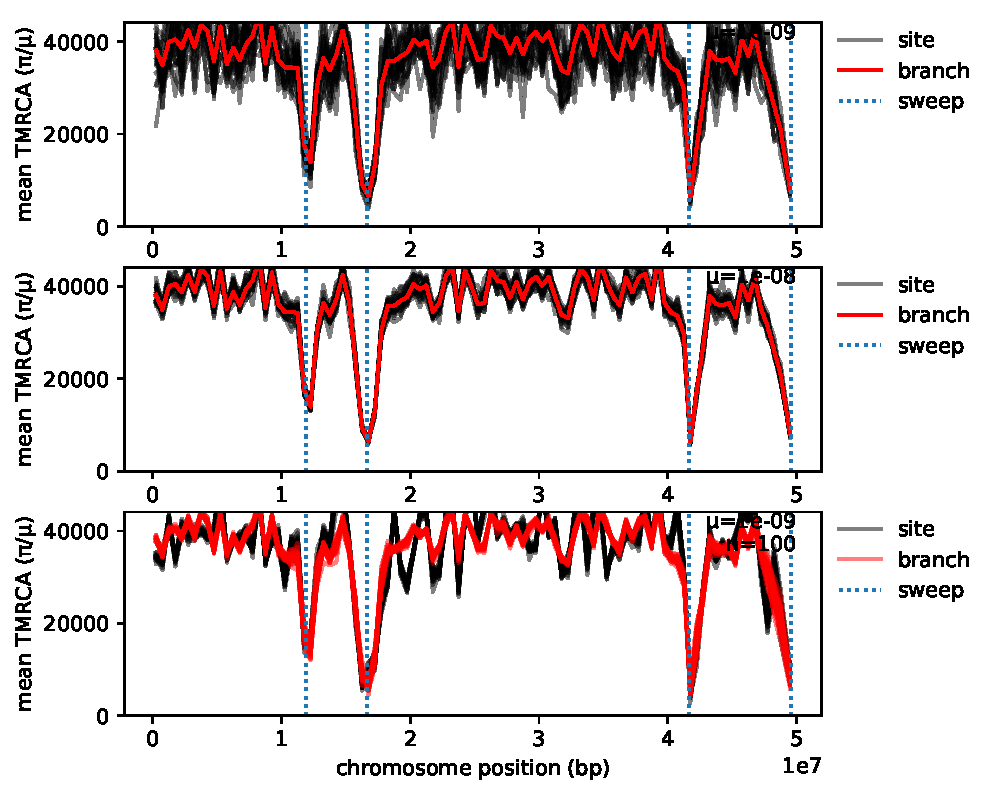
\includegraphics{{figures/swept.10000.765.1e-09.diversity}.pdf}
    \caption{
        As in Figure~\ref{fig:sweep_duality}, but in a population of size 10,000.
        \label{sfig:sweep_duality_10K}
    }
\end{figure}

\begin{figure}
    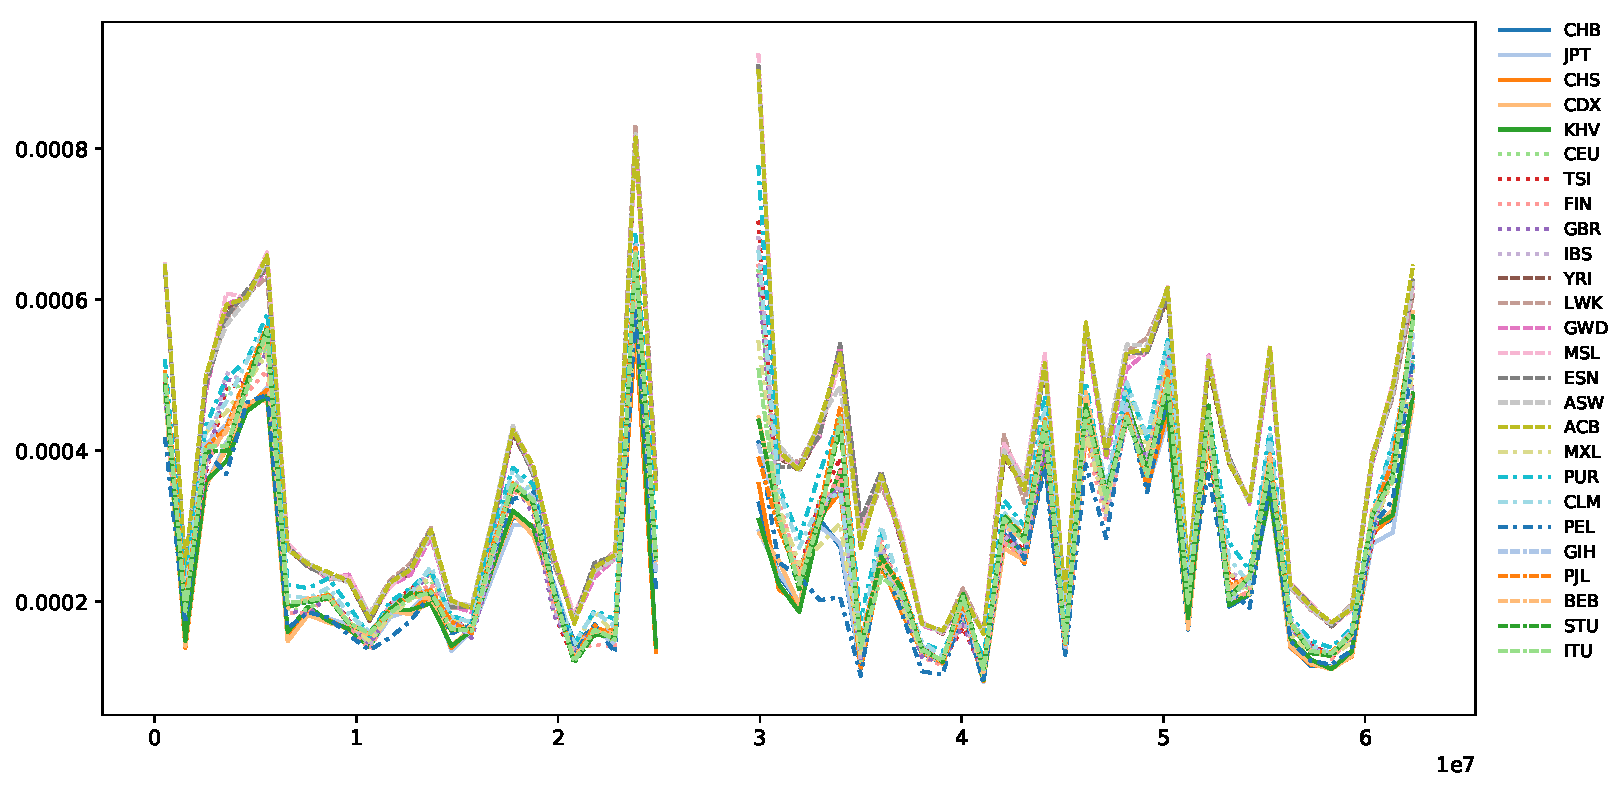
\includegraphics[width=0.5\textwidth]{{figures/1kg/relate_chr20.site.1000000.diversity}.pdf}
    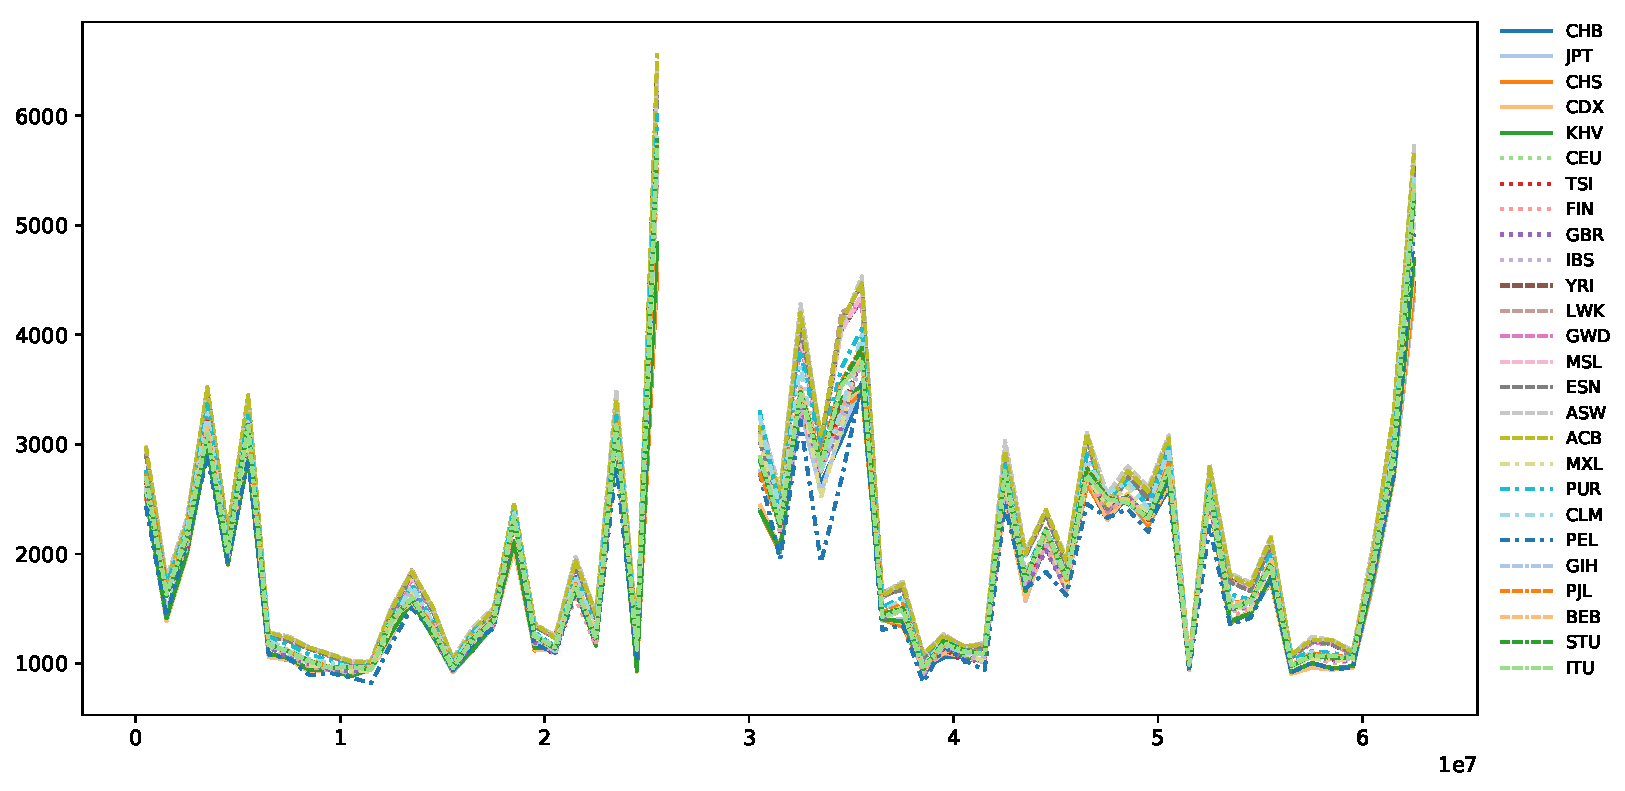
\includegraphics[width=0.5\textwidth]{{figures/1kg/1kg_chr20.branch.1000000.diversity}.pdf}
    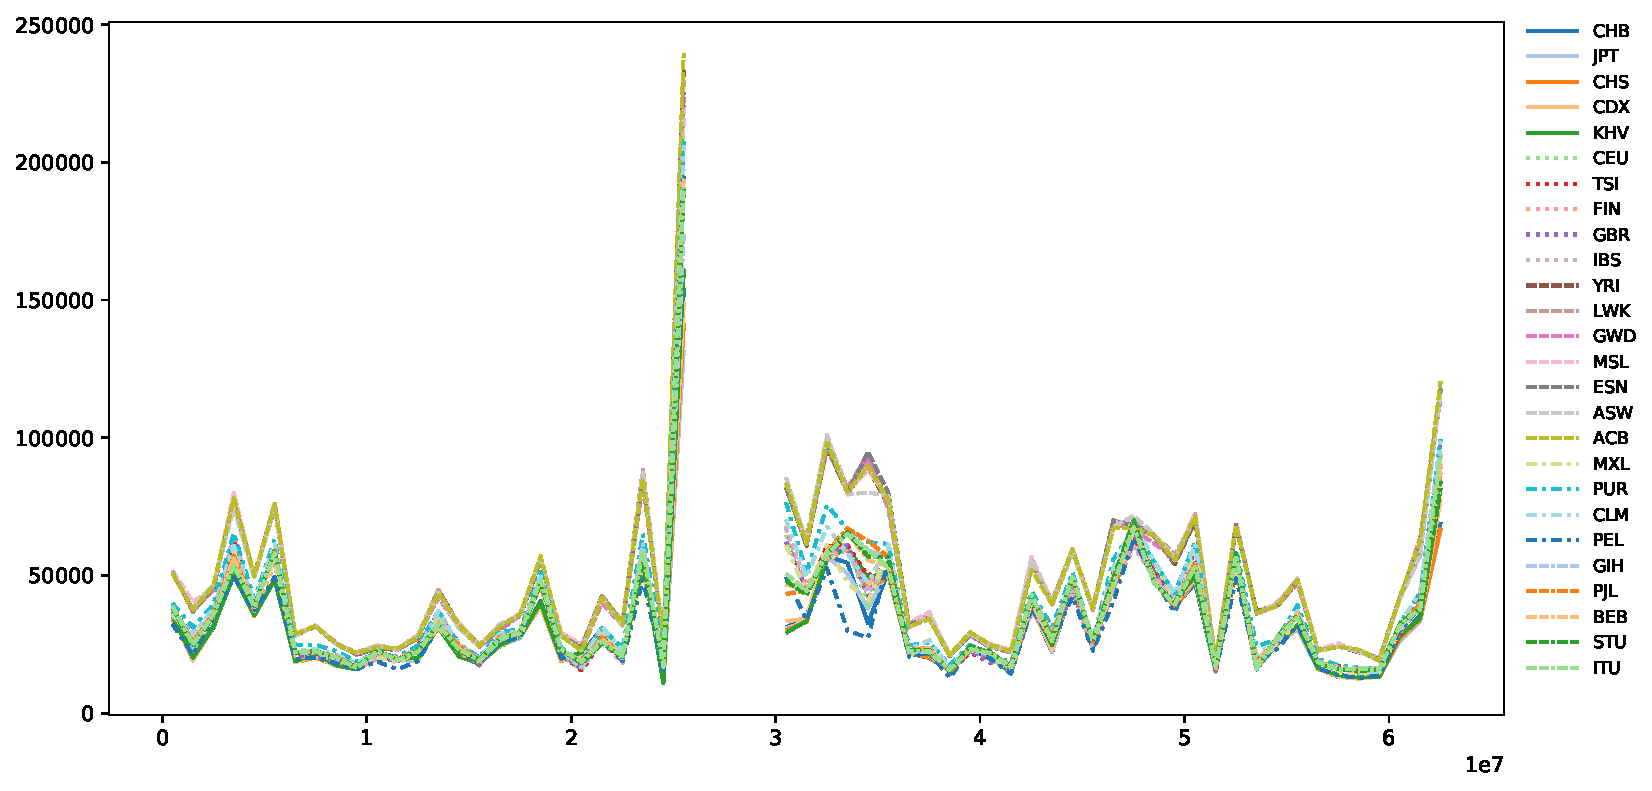
\includegraphics[width=0.5\textwidth]{{figures/1kg/tgp_geva_chr20.branch.1000000.diversity}.pdf}
    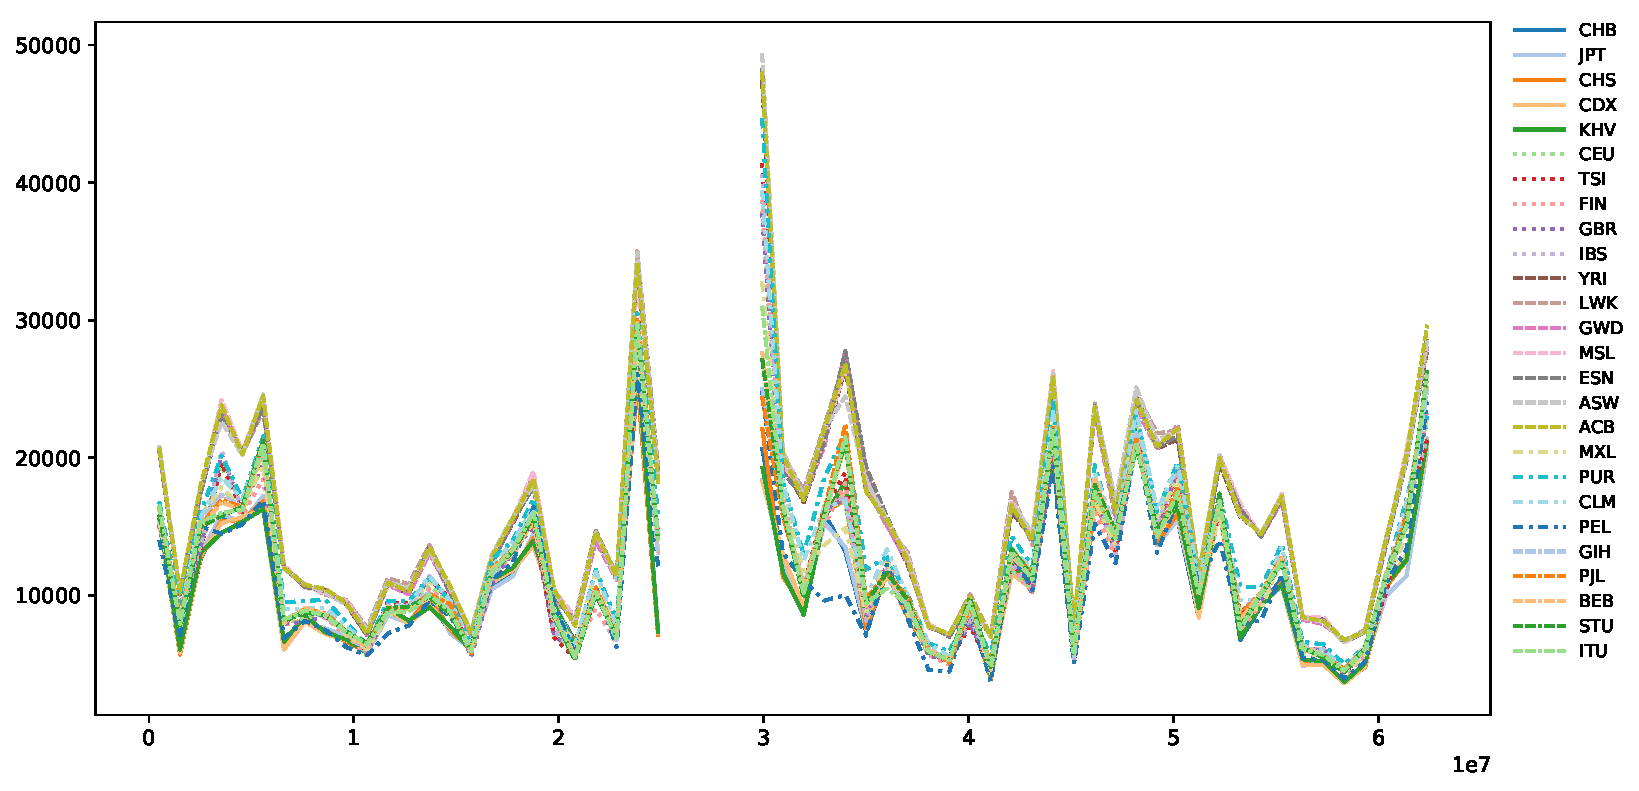
\includegraphics[width=0.5\textwidth]{{figures/1kg/relate_chr20.branch.1000000.diversity}.pdf}
    \caption{
        \textbf{(top left)} Mean sequence diversity
        in 1Mb windows along human chromosome 20 of the 1000 Genomes Project,
        and the dual branch statistic as calculated from tree sequences inferred by
        \textbf{(top right)} \tsinfer,
        \textbf{(bottom left)} GEVA, and
        \textbf{(bottom right)} Relate.
        \label{fig:chr20_full}
    }
\end{figure}



\end{document}


%%%%%%%%%%%%%%%%%%
\subsection*{Genomic PCA}

Let $G$ denote the genotype matrix, so that $G_{ja} \in \{0,1\}$
is the genotype of the $a^\text{th}$ individual
at the $j^\text{th}$ site, with `1` denoting the derived state
(we assume here biallelic markers).
Also let $P_j = (1/n) \sum_a G{ja}$ denote the vector of allele frequencies.
Then the \emph{genetic covariance} between samples $a$ and $b$ is
\begin{align*}
    C_{ab}
        &= \frac{1}{L} \sum_j (G_{ja} - P_j) (G_{jb} - P_j) . %  \\
        % &= \frac{1}{L} \left( (G - P \bone^T)^T (G - P \bone^T) \right)_{ab} .
\end{align*}
This can be computed by letting
$\iw_a = \delta_a$ and $\iw_b = \delta_b$
(these weights mark nodes ancestral to $a$ and $b$ respectively)
and $\iw_t = \bone / n$
(this weight gives the proportion of samples inheriting from each node).
Then, with
$f(\nw_a, \nw_b, \nw_t) = (\nw_a - \nw_t) (\nw_b - \nw_t)$,
we can compute the covariance as
\begin{align*}
    C_{ab} = \frac{1}{2} \bar \site(f, (\iw_a, \iw_b, \iw_t)) .
\end{align*}
This follows, including the factor of two,
because the summary function applied to the ancestral allele
at a site with derived allele frequencies $p_a$, $p_b$, and $p_t$
in sample $a$, sample $b$, and total, respectively, is
$f(1 - p_a, 1 - p_b, 1 - p_t) = f(p_a, p_b, p_t)$.

Computing the full covariance matrix for a large number of samples may be infeasible.
However, we can efficiently find $y^T C z$ for arbitrary vectors $y$ and $z$.
This works because if we set the initial weights to $y$,
then each allele's weight is equal to the sum of the entries of $y$
corresponding to samples carrying that allele.
Then, if we define
$f_{yz}(u, v, t) = (u - (\sum_a y_a) t) (v - (\sum_b z_b) t)$,
then
\begin{align} \label{eqn:yCz}
    \frac{1}{2} \bar \site(f_{yz}, (y, z, \iw_t))
        &= \frac{1}{L} \sum_j (\sum_a y_a G_{ja} - (\sum_a y_a) P_j)
                    (\sum_b z_b G_{jb} - (\sum_b z_b) P_j) \\
        &= y^T C z .
\end{align}

\plr{Hmph: to actually compute $Cz$ we need one weight vector for each sample, again.
    TODO: look up if you can do Krylov just by computing $y^t C z$ for a reasonable number of vectors.
    We could compute $Cz$ quickly if we could propagate down the tree:
    we'd have $(Cz)_a$ equal to the sum of the weights at all nodes \emph{ancestral to} $a$. }

Where does the signal from an eigenvector come from?
Let $y$ be an eigenvector of $C$ with eigenvalue $\lambda$, normalized so that $\|y\|^2 = 1$.
Since $Cy = \lambda y$,
we can write $1 = \sum_a y_a^2 = (1/\lambda) y^T C y$.
However, equation \eqref{eqn:yCz} gives $y^T C y$ as a sum over \emph{sites},
and thus distributes the variance in $G$ associated with $y$
across the tree sequence.
(This is true because of the singular value decomposition of $G$.)

\paragraph{Diploid statistics}
The statistics we develop here are in essence \emph{haploid} statistics.
These tools can be used to compute a statistic about polyploid individuals,
but they do not scale to large numbers of individuals.
For instance, to compute the heterozygosity of a set of samples
-- this is $(1/N) \sum_{i=1}^N 2 p_i (1-p_i)$, where $p_i$ is the derived allele frequency
in the $i^\text{th}$ individual --
one would need to have an entry in the weight vector for \emph{each individual}.
The genotype of a diploid at a site with a single mutation that occurred on the branch ancestral to node $n$
is determined by where that node falls relative to the diploid's two haplotypes in the tree:
if $n$ is on the path from either haplotype to their MRCA, the individual is heterozygous;
if $n$ is on the path from the MRCA to the root, the individual is homozygous derived;
and the individual is homozygous ancestral otherwise.
This suggests the following generalization of our current scheme for diploids:
for a list $(I_1, \ldots, I_N)$ of pairs of nodes,
and two vectors $w^{(1)}$ and $w^{(2)}$ of weights of length $N$,
add weight $w^{(1)}_i$ to each node on the path between the two nodes of $I_i$,
and weight $w^{(2)}_i$ to each node on the path from the MRCA of $I_i$ to the root.
With $k$ such weighting schemes, we would then need the summary function $F$
to take $k \times 2$ values as input.
Efficiently updating these ``diploid'' weights on the nodes should be possible,
but is not a straightforward extension of our current method.
